\chapter{Non-Uniform Dependence and Well-posedness for 
HR}
\section{Introduction}
%
We consider the  initial value problem for
the hyperelastic rod (HR)  equation
%
%
\begin{align}
\label{hr}
& \p_t u
-
\p_t \p_x^2 u
+
3u\p_x u
=
\gamma \big (
2\p_x u \p_x^2 u
+
u \p_x^3 u
\big ),
\\
\label{hr-data}
& u(x, 0) = u_0 (x),
\quad x  \in \ci, \text{  or  } \rr \quad t \in \rr,
\end{align}
%
%
%
%
%
%
where  $\gamma$  is a  nonzero constant,
and prove that the dependence of solutions on initial data is not uniformly 
continuous in Sobolev spaces $H^s(\ci)$, $s>3/2$.
Thus, we extend the result proved by Olson 
\cite{Olson_2006_Non-uniform-dep} in the periodic
case (for $s\ge 2$ and $\gamma \ne 3$)  to  $s>3/2$ (the entire 
well-posedness range)
for HR. Furthermore,  motivated by the work of
 Himonas  and Kenig \cite{Himonas:2009fk},
we establish non-uniform dependence
in the non-periodic case, where the method of traveling wave solutions used in  
\cite{Olson_2006_Non-uniform-dep} does not seem to work.
%
%

The HR equation was first
derived by Dai in \cite{Dai_1998_Model-equations} as a one-dimensional 
model for finite-length and
small-amplitude axial deformation waves in thin cylindrical
rods composed of a compressible Mooney-Rivlin
material. The derivation relied upon a reductive perturbation technique, 
and took into account the nonlinear dispersion of pulses propagating 
along a rod. It was assumed that each cross-section of the rod is 
subject to a stretching and rotation in space. The solution $u(x,t)$ to the 
HR equation represents the radial stretch relative
to a pre-stressed state, while $\gamma$ is a fixed constant depending upon 
the pre-stress and the material used in
the rod, with values ranging from $- 29.4760$ to $3.4174$.

%
The well-posedness of the HR equation has been studied by several authors. 
In Yin \cite{Yin_2003_On-the-Cauchy-p} and Zhou 
\cite{Zhou_2005_Local-well-pose}, a proof of local well-posedness in Sobolev 
spaces $H^s$,  $s > 3/2$, is described  on the line and the circle, respectively. 
Their approach is to rewrite the HR equation   
in its non-local form, and then to verify the conditions needed to apply 
Kato's semi-group theory \cite{Kato_1975_Quasi-linear-eq}. 
For details on how this is done for CH on the line, see Rodriguez-Blanco 
\cite{Rodriguez-Blanco_2001_On-the-Cauchy-p}. Blow-up criteria 
is also investigated in \cite{Yin_2003_On-the-Cauchy-p} and 
\cite{Zhou_2005_Local-well-pose}, as well as by Constantin and Strauss 
\cite{Constantin_2000_Stability-of-a-}. 


Setting $\gamma = 0$ gives the celebrated 
BBM equation, which was proposed by 
Benjamin, Bona, and Mahony 
\cite{Benjamin_1972_Model-equations} as a model for 
the unidirectional evolution of long waves.
Solitary-wave solutions to this 
equation are global and orbitally stable (see Benjamin 
\cite{Benjamin_1972_The-stability-o}, 
\cite{Benjamin_1972_Model-equations}, and 
\cite{Constantin_2000_Stability-of-a-}).
For more general $\gamma$, the existence of global 
solutions to HR on the line with constant $H^1$ energy
was proved recently by Mustafa \cite{Mustafa_2007_Global-conserva}
using the approach developed by Bressan and 
Constantin in \cite{Bressan_2007_Global-conserva}. Using a vanishing 
viscosity argument, Coclite, 
Holden, and Karlsen \cite{Coclite_2005_Global-weak-sol}
established existence of a strongly continuous semigroup of global 
weak solutions of HR on the line for initial data in $H^1$.
Bendahmane, Coclite, and Karlsen 
\cite{Bendahmane_2006_Hsp-1-perturbat} extended this result to traveling 
wave solutions that are supersonic solitary shockwaves.
For more information on the existence of global solutions to the HR
equation, see Holden and Raynaud \cite{Holden_2007_Global-conserva}
and \cite{Yin_2003_On-the-Cauchy-p}. 

There is a variety of traveling wave solutions to the HR equation that can be 
obtained using various combinations of peaks, cusps, compactons, 
fractal-like waves, and plateaus (see Lenells 
\cite{Lenells_2006_Traveling-waves}). Orbital stability of solitary wave 
solutions was proved in \cite{Constantin_2000_Stability-of-a-}.
Solitary shock wave formation was 
analyzed in Dai and Huo \cite{Dai_2000_Solitary-shock-} using traveling 
wave solutions of the HR equation to derive a system of ordinary differential 
equations, with a vertical singular line in the phase plane corresponding with the 
formation of shock waves. Head-on collisions between two solitary 
waves was investigated in the work of Hui-Hui Dai, 
Shiqiang Dai, and Huo \cite{Dai_2000_Head-on-collisi} using a reductive 
perturbation method coupled with the technique of strained coordinates. 

In this work we study the continuity of the data-to-solution map for the HR 
equation.
Using the method of traveling wave solutions it was shown in  
\cite{Olson_2006_Non-uniform-dep} that the data-to-solution map
$u_0  \mapsto u$ of the periodic HR equation is not uniformly continuous 
from any bounded set in $H^s(\ci)$ into $C([0, T ], H^s(\ci))$ for $s \ge 
2$ and $\gamma \neq 3$. Non-uniform dependence for the non-periodic CH 
equation in 
$H^s(\rr)$ for $s>1$ was proven in \cite{Himonas:2009fk} 
using the method of approximate solutions and well-posedness estimates. The 
case $s=1$ for both the line and the circle
 was proved earlier by Himonas, Misiolek, and Ponce in 
 \cite{Himonas_2007_Non-uniform-con}.
 Recently  in \cite{Himonas_2009_Non-uniform-dep-per} non-uniform 
 continuity of the solution map for the CH equation
 on the circle has been proved
 for the whole range of Sobolev exponents for which local well-posedness of 
 CH is known.
 
 We mention that the continuity of the data-to-solution map  for CH has 
 been studied in  \cite{Himonas_2007_Non-uniform-con},
 \cite{Himonas_2001_The-Cauchy-prob}, and 
 \cite{Himonas:2005kx}, and for the Euler equations in 
 \cite{Himonas_2009_Non-uniform-dep-euler}. Continuity of this map for  
 the  Benjamin-Ono equation was studied in  Koch and  Tzvetkov 
 \cite{Koch_2005_Nonlinear-wave-}. For related ill-posedness results, we 
 refer the reader to Kenig, Ponce, and  Vega 
 \cite{Kenig_2001_On-the-ill-pose}, Christ, Colliander, and Tao 
 \cite{Christ_2003_Asymptotics-fre}, and the references 
 therein.

Here we consider the initial value problem for the HR equation
in both the periodic and non-periodic cases
and prove non-uniform  continuity of the solution map. 
More precisely, we show the following result:
%
%%%%%%%%%%%%%%%%%%%%%%%%
%
%
%    Theorem:  hr-non-unif-dependence
%
%
%%%%%%%%%%%%%%%%%%%%%
%
\begin{theorem}
\label{hr-non-unif-dependence}
Let $\gamma$ be a nonzero constant. Then 
the data-to-solution map $u(0) \mapsto u(t)$ of the Cauchy-problem
for the HR equation
\eqref{hr}-\eqref{hr-data}
is not uniformly continuous
from any bounded subset of  $H^s$ into $C([-T, T], H^s)$
for $s>3/2$ on the line and circle.
%
\end{theorem}
%
%
%
As we mentioned above, when  $\gamma=0$ the HR equation
 becomes the BBM equation.
 Bona and Tzvetkov \cite{Bona_2009_Sharp-well-pose} have recently proved  that this equation  
is globally well-posed in  Sobolev spaces $H^s$, if $s \ge 0$,
and that its data-to-solution map is smooth.

%
Our approach  for proving \cref{hr-non-unif-dependence}  
mirrors  that in Himonas and Kenig \cite{Himonas:2009fk} and 
Himonas, Kenig, and Misiolek \cite{Himonas_2009_Non-uniform-dep-per}.
That is, we will choose 
approximate solutions to the HR equation such that the size of the difference between approximate and actual solutions with 
identical initial data is negligible. Hence, to understand the degree of 
dependence, it will suffice to focus on the behavior of the approximate 
solutions (which will be simple in form), rather than on the behavior of the 
actual solutions. In order for the method to go through, we will 
need well-posedness estimates for  the size of the 
actual solutions to the HR equation, as well a 
lower bound for their lifespan. This will permit us to obtain an upper 
bound for the size of the difference of approximate and actual solutions. 
More precisely, we will need the following well-posedness result  with estimates,  
stated in both the  periodic and non-periodic case:


%%%%%%%%%%%%%%%%%%%%%%%%
%
%            wp of theorem in R and T
%
%%%%%%%%%%%%%%%%%%%%%%%%
%
%
%
%
\begin{theorem}
\label{thm:HR_existence_continuous_dependence}
If   $s>3/2$  then we have:

(i) If $u_0\in H^s$  then  there exists a unique solution to
the Cauchy problem  \eqref{hr}--\eqref{hr-data} in $C([-T, T], H^s)$, where 
the lifespan  $T$ depends on the size
of the initial data $u_0$. Moreover, 
the  lifespan $T$ satisfies the lower bound estimate 
%
%
%
\begin{equation}
\label{Life-span-est}
T
\ge
\frac{1}{2c_s \|u_0\|_{H^s}}.
\end{equation}
%

(ii)
The flow map $u_0 \mapsto u(t)$ is continuous from
bounded sets of $H^s$ into \\ $C([-T, T], H^s)$,
and the solution $u$ satisfies the estimate
%
%
%
\begin{equation}
\label{u_x-Linfty-Hs}
\|
u(t)
\|_ {H^s}
\le
2
\|
u_0
\|_{H^s}, \ \ |t|\le T.
\end{equation}
%
%
%
\end{theorem}
%
%
A proof of existence, uniqueness, and continuous dependence in this 
theorem for $\gamma =1$ (CH) 
is given  by Li and Olver in 
\cite{Li_2000_Well-posedness-} using a regularization method, and in
\cite{Rodriguez-Blanco_2001_On-the-Cauchy-p} using 
Kato's semi-group method \cite{Kato_1975_Quasi-linear-eq}. As mentioned 
above, proofs of 
existence, uniqueness, and continuous dependence for  HR
have been outlined in \cite{Yin_2003_On-the-Cauchy-p} and 
\cite{Zhou_2005_Local-well-pose} for the line and circle, 
respectively. Both outlines rely upon an application of Kato's semi-group 
method. However, we have not been able to find estimates  
\eqref{Life-span-est} and \eqref{u_x-Linfty-Hs}  in the literature.
Here we shall give a proof of local well-posedness of HR,
including  estimates \eqref{Life-span-est} and \eqref{u_x-Linfty-Hs},
which are key ingredients in our work, 
following an alternative approach used for nonlinear hyperbolic equations
in Taylor \cite{Taylor_1991_Pseudodifferent}.

\hrule
\textbf{Furthermore, following \cite{Chen:2011fk}, we expand upon our non-uniform
dependence results by studying the data-to-solution map in a weaker topology.
More precisely, we show the following result:}
\hrule
%
%
\begin{theorem}
For $\gamma \neq 0$, the
data to solution map for HR is H\"older continuous from $B_{H^{s}}(R)$ (measured
in $H^{r}$) to $C([0, T], H^{r})$, where $T = T(R)$, for $s > 3/2$, $-1 \le r <
s$. More precisely, decompose the set $\Omega = \left\{ (s, r) \in \rr^{2}
\right\}$ into the pieces
  %
  %
  \begin{equation*}
  \begin{split}
    & \Omega_{1} = \left\{ (s, \ r):  \ s < 3/2 \right\}
    \\
    & \Omega_{2} = \left\{ (s, \ r):
     \ s>3/2, \ r < -1  \right\}
    \\
    & \Omega_{3} = \left\{ (s, \ r):
     \ s>3/2, \ r > s  \right\}
    \\
    & \Omega_{4} = \left\{ (s, \ r):
     \ s>3/2, \ -1 \le r \le s-1, \ s + r \ge 2  \right\}
    \\
    & \Omega_{5} = \left\{ (s, \ r):
     \ s>3/2, \ -1 \le r < 2-s \right\}
    \\
    & \Omega_{6} = \left\{ (s, \ r):
    \  s>3/2, \  s-1 < r < s  \right\}.
    \end{split}
\end{equation*}
  %
  %
\label{thm:main-thm}
\end{theorem}
%
\begin{center}
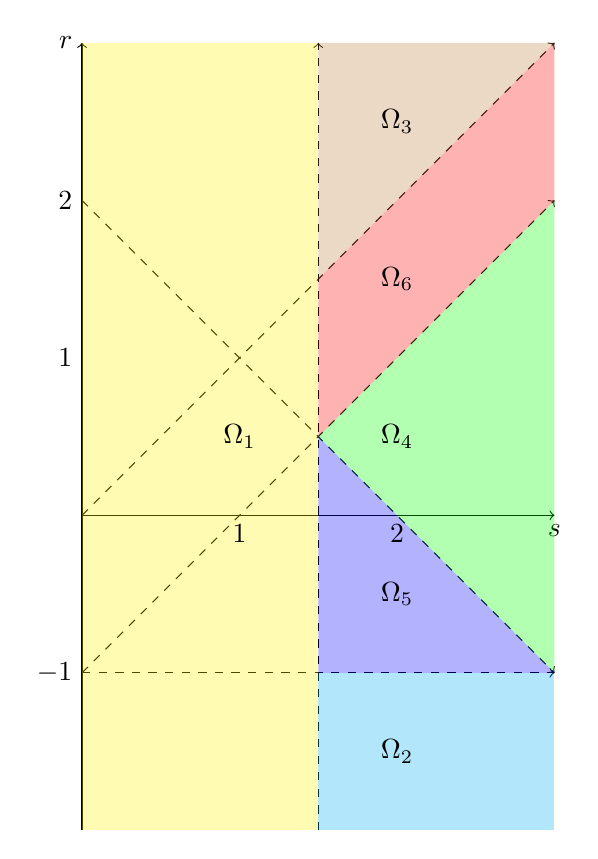
\begin{tikzpicture}[scale=2]
% Draw thin grid lines with color 40% gray + 60% white

% Draw x and y axis lines
\draw [->] (0,0) -- (3,0) node [below] {$s$};
\draw [->] (0,-2) -- (0,3) node [left] {$r$};
\draw [->, dashed] (0,0) -- (3,3);
\draw [->, dashed] (0,-1) -- (3,2);
\draw [->, dashed] (0,2) -- (3,-1);
\draw [->, dashed] (0,-1) -- (3,-1);
\draw [->, dashed] (3/2,-2) -- (3/2, 3);
\fill[color=green, fill opacity=0.3] (1.5, 0.5) -- (3,2) -- (3,0) -- (3,-1);
\fill[color=red, fill opacity=0.3] (1.5, 0.5) -- (1.5,1.5) -- (3,3) -- (3,2);
\fill[color=yellow, fill opacity=0.3] (0, -2) -- (1.5, -2) -- (1.5, 3) -- (0, 3);
\fill[color=blue, fill opacity=0.3] (1.5, 0.5) -- (1.5, -1) -- (3, -1);
\fill[color=brown, fill opacity=0.3] (1.5, 1.5) -- (3, 3) -- (1.5, 3);
\fill[color=cyan, fill opacity=0.3] (1.5, -1) -- (3, -1) -- (3, -2) -- (1.5, -2);


\foreach \x/\xtext in {1, 2}
    \draw[shift={(\x,0)}]  node[below] {$\xtext$};
\foreach \y/\ytext in {-1, 1, 2}
    \draw[shift={(0,\y)}]  node[left] {$\ytext$};
    \draw (1,0.5) node {$\Omega_{1}$};
    \draw (2,2.5) node {$\Omega_{3}$};
    \draw (2,1.5) node {$\Omega_{6}$};
    \draw (2,-1.5) node {$\Omega_{2}$};
    \draw (2,0.5) node {$\Omega_{4}$};
    \draw (2,-0.5) node {$\Omega_{5}$};
\end{tikzpicture}
\end{center}
%
%
Then for two initial data $u_{0}, v_{0} \in B_{H^{s}}(R)$, there exist unique
corresponding solutions $u(x,t), v(x,t)$ for $0 \le t \le T= T(R)$ to the
HR equation \eqref{hyperelastic-rod-equation} which satisfy 
%
%
\begin{equation*}
\begin{split}
  \| u(t) - v(t) \|_{H^{r}} \le C \| u_{0} - v_{0} \|_{H^{r}}^{\alpha(s, r)},
  \quad 0
  \le t \le T
\end{split}
\end{equation*}
%
%
where 
%
%
\begin{equation*}
\begin{split}
\alpha = 
\begin{cases}
   1, \quad & (s,r) \in \Omega_{4} 
  \\
   2(s-1)/(s-r),  \quad & (s, r) \in \Omega_{5}
  \\
   s-r, \quad & (s, r) \in \Omega_{6}.
\end{cases}
\end{split}
\end{equation*}
%


This work is structured as follows. In \cref{sec:2} we prove 
\cref{hr-non-unif-dependence} on the line and 
in \cref{sec:3} we prove it on the circle.
As mentioned above, we begin with two sequences of
appropriate approximate solutions and then 
we construct  actual solutions
coinciding at time zero  with the approximate solutions.
The key step is to show that  the $H^s$-size of
the difference between approximate and actual solutions 
converges to zero (see propositions \ref{applelem:bound_for_difference-of-approx-and-actual-soln}
and  \ref{prop:bound_for_difference-of-approx-actual-soln}). 
In \cref{sec:4} we  prove 
\cref{thm:HR_existence_continuous_dependence} 
using a Galerkin-type argument and energy estimates.
In \cref{sec:pf-holder}, we provide the proof of Theorem \ref{thm:main-thm}.

%
%
%
%	
%
%
%
%
%%%%%%%%%%%%%%%%%%%%%%%%
%
%           Proof of  \cref on the line
%
%%%%%%%%%%%%%%%%%%%%%%%%
%
%
%
%
%
\section{Proof of Non-Uniform Dependence on the line
}
\label{sec:2}
%
%
%
%
We begin by outlining the method of the proof,
as it has been applied for the case $\gamma=1$ in \cite{Himonas:2009fk}.
We will show  that there there exist two sequences of solutions 
$u_n(t)$
and $v_n(t)$ in $C([-T, T], H^s)$ such that
%
%
%
%
\begin{equation}
\label{h-s-bdd}
\| u_n(t)  \|_{H^s}
+
\| v_n(t)  \|_{H^s}
\lesssim
1,
\end{equation}
%
%
%
%
%
\begin{equation}
\label{zero-limit-at-0}
\lim_{n\to\infty}
\|
u_n(0)
-
v_n(0)
\|_{H^s}
=
0,
\end{equation}
%
%
%
%
and
%
%
%
%
\begin{equation}
\label{bdd-away-from-0}
\liminf_{n\to\infty}
\|
u_n(t)
-
v_n(t)
\|_{H^s}
\gtrsim
|\sin ( \gamma t)|,
\quad
| \gamma t|\le 1.
\end{equation}%
%
%
We accomplish this in two steps.
First, we will construct two sequences of approximate solutions
satisfying the above properties.
Then, we will construct two sequences of actual solutions 
coinciding with the approximate solutions at time zero.
The key point of this method is that 
the difference between solutions and approximate solutions
must decay.

%
%
For this method, it is more convenient 
to rewrite the Cauchy problem for the HR equation 
in the following non-local form
%
%
\begin{align}
& \p_t u =  -\gamma u \p_x u -
\Lambda^{-1} \left[ \frac{3-\gamma}{2}u^2 +
\frac{\gamma}{2} \left( \p_x u \right)^2
\right],
\label{apple1'}
\\
&  u(x,0) = u_0(x), \; \; x \in \rr, \; \; t \in \rr
\label{apple2'}
\end{align}
%
%
where 
\begin{equation*}
	\Lambda^{-1} = \p_x (1 - \p_x^2)^{-1}.
\end{equation*}
%
%
%
%
%
%
\textbf{Approximate solutions.}
Following \cite{Himonas:2009fk}, our approximate solutions
\\ $u^{\omega, \lambda} = u^{\omega,
\lambda}(x,t)$ to \eqref{apple1'}-\eqref{apple2'} will
consist of a low frequency and a high frequency part,
i.e.
%
%
%
%
\begin{equation}
\label{apple1}
u^{\omega,\lambda} = u_\ell + u^h
\end{equation}
%
%
%
%
where $\omega$ is in a bounded set of $\rr$ and $\lambda > 0$. The high frequency part is given by 
%
%
%
%
\begin{equation}
\begin{split}
u^h = u^{h,\omega,\lambda}(x,t) =
\lambda^{-\frac{\delta}{2} -s}
\phi \left (\frac{x}{\lambda^\delta}\right )
\cos(\lambda x - \gamma \omega t)
\end{split}
\end{equation}
%
%
%
%
where $\phi$ is a $C^\infty$ cut-off function such that
%
%
%
%
\begin{equation*}
\phi = \begin{cases}
1, &\text{if $|x|<1$,} \\
0, &\text{if $|x| \ge 2,$} \end{cases}
\end{equation*}
%
%
%
%
and by \cref{thm:HR_existence_continuous_dependence} 
we let the low frequency part $u_\ell = u_{l,
\omega, \lambda}(x,t)$ be the unique solution to the Cauchy problem
%
%
\begin{align}
\label{u-l-apple1'}
& \p_t u_\ell = -\gamma u_\ell \p_x u_\ell -
\Lambda^{-1} \left[ \frac{3-\gamma}{2}(u_\ell)^2 +
\frac{\gamma}{2} \left( \p_x u_\ell \right)^2
\right],
\\
& u_\ell(x,0) = \omega \lambda^{-1} \tilde{\phi} \left(
\frac{x}{\lambda^{\delta}}
\right), \quad x \in \rr, \quad t \in \rr
\label{apple1**}
\end{align}
%
%
%
%
where $\tilde{\phi}$ is a $C^{\infty}_0(\rr)$ function such that
%
%
%
%
\begin{equation}
\label{apple1***}
\tilde{\phi}(x) = 1 \; \;  \text{if} \; \;
x \in \text{supp} \; \phi.
\end{equation}
%
%
%
%
We remark that for $\lambda >>1$ and $\delta < 2$ the approximate solutions 
$u^{\omega, \lambda}$ share a common lifespan $T >> 1$. To see why, we 
first note that the high frequency part $u^{h, \omega, \lambda}$ has 
infinite lifespan by the following, whose 
proof can be found in \cite{Himonas:2009fk}: 
%
%
\begin{lemma}
\label{applea}
Let $\psi \in S(\rr)$, $\alpha \in \rr$. Then for $s \ge 0$ we have
%
%
\begin{equation}
\begin{split}
\lim_{\lambda \to \infty} \lambda^{-\frac{\delta}{2}-s}
\|\psi \left( \frac{x}{\lambda^\delta} \right)\cos(\lambda
x - \alpha) \|_{H^s(\rr)} = \frac{1}{\sqrt
2}\|\psi\|_{L^2(\rr)}.
\label{apple6}
\end{split}
\end{equation}
%
%
Relation \eqref{apple6} remains true if $\cos$ is
replaced by $\sin$.
\end{lemma}
%
%
For the low frequency part $u_{\ell, \omega, \lambda}$, we apply \eqref{Life-span-est} and the estimate
%
%
\begin{equation}
\begin{split}
	\label{tildphi}
\|\tilde{\phi}\left( \frac{x}{\lambda^\delta}
\right)\|_{H^{k}(\rr)} \le
\lambda^{\frac{\delta}{2}}\|\tilde{\phi}\|_{H^{k}(\rr)},
\quad k\ge 0
\end{split}
\end{equation}
%
%
to obtain a lower bound for its lifespan
%
\begin{equation*}
	\label{lifespan-bound-1}
	\begin{split}
		T_{\ell, \omega,\lambda} \ge \frac{1}{2 c_s \|u_{\ell, \omega, \lambda}(0)\|_{H^s(\rr)}} = 
		\frac{1}{2 c_s |\omega|
		\lambda^{\frac{\delta}{2}-1}\|\tilde{\phi}\|_{H^s(\rr)}} >> 1.
	\end{split}
\end{equation*}
%
%
Since $\omega$ belongs to a bounded subset of $\rr$, the existence of a 
common lifespan $T >> 1$ follows. 
%
%

Substituting the
approximate solution $u^{\omega, \lambda} = u_\ell + u^h$ into the HR
equation, we see that the error
$E$ of our approximate solution is given by
%
%
\begin{equation*}
E=E_1 + E_2 + \dots + E_8
\end{equation*}
%
%
where
%
%
\begin{equation}
\label{all_errors_together}
\begin{split}
E_1 & = \gamma \lambda^{1 -\frac{\delta}{2}-s}  \left[ u_\ell(x,0) - u_\ell(x,t)
\right] \phi\left(
\frac{x}{\lambda^ \delta}
\right)\sin(\lambda x - \gamma \omega t),
\\
E_2 & = \gamma \lambda^{-\frac{3\delta}{2}-s}
u_\ell(x,t) \cdot \phi'\left( \frac{x}{\lambda^\delta} \right)\cos\left( \lambda
x - \gamma \omega t
\right),
\\
E_3 & = \gamma u^h \p_x u_\ell, \; \; E_4 = \gamma u^h \p_x u^h, \ E_5  = 
 \frac{3-\gamma}{2} \Lambda^{-1} \left[  \left( u^h \right)^2 \right], \\
E_6 & = (3- \gamma)\Lambda^{-1}
  \left[ u_\ell u^h \right], \  E_7 = \frac{\gamma}{2} \Lambda^{-1} \left[ 
 \left(
\p_x u^h \right)^2 \right ], \; \;
E_8 = \gamma \Lambda^{-1} \left[  \p_x u_\ell \p_x u^h \right]
.
\end{split}
\end{equation}
%
%
%
Next we prove the decay of the error:
%
%
\begin{proposition}
Let $1<\delta<2$. Then for $s > 1$, bounded $\omega$, and
$\lambda >>1$ we are assured the decay of the error $E$ of the
approximate solutions to the HR equation. Specifically
%
%
%
\begin{equation}
\label{E-est}
\|E(t)\|_{H^1(\rr)} \lesssim \lambda^{\frac{\delta}{2} -s}, \quad |t| \le 
T.
\end{equation}
%
%
%
\end{proposition}
%
%
%
\textbf{Proof.}
It will suffice to estimate the $H^1$ norms of each $E_i$.
Here we estimate only $E_1$. 
The remaining error terms are estimated 
like in \cite{Himonas:2009fk} for the case $\gamma=1$.
We have
%
%
\begin{equation}
	\label{fw-est}
\begin{split}
\|E_1\|_{H^1(\rr)}
& = \| \gamma \lambda^{1 -\frac{\delta}{2}-s} \left[ u_\ell(x,0) - u_\ell(x,t) \right]
 \phi\left( \frac{x}{\lambda^\delta}
\right ) \sin (\lambda x - \gamma \omega t )\|_{H^1(\rr)}
\\
& \lesssim \lambda^{1 -\frac{\delta}{2} -s } \|\left[ u_\ell(x,0) - 
u_\ell(x,t)
\right] \phi\left( \frac{x}{\lambda^\delta} \right )
\sin\left( \lambda x - \gamma \omega t
\right) \|_{H^1(\rr)}.
\end{split}
\end{equation}
%
%
Applying the inequality 
%
%
\begin{equation*}
\label{applec}
\|fg\|_{H^1(\rr)} \le \sqrt{2} \|f\|_{C^1(\rr)} \|g\|_{H^1(\rr)}
\end{equation*}
%
%
%
%
%
%
%
%
to estimate \eqref{fw-est} gives
%
%
\begin{equation}
\begin{split}
\|E_1\|_{H^1(\rr)} \lesssim \lambda^{1 - \frac{\delta}{2} -s } \|\phi
\left( \frac{x}{\lambda^\delta} \right) \sin (\lambda x - \gamma \omega t)
\|_{C^1(\rr)} \|[u_\ell (x,0) - u_\ell (x,t) ] \|_{H^1(\rr)}.
\label{apple14}
\end{split}
\end{equation}
%
%
We now estimate the right-hand side of \eqref{apple14} in pieces. First, 
note that routine computations give
%
%
\begin{equation}
\begin{split}
\|\phi\left( \frac{x}{\lambda^\delta} \right) \sin(\lambda x - \gamma 
\omega t)
\|_{C^1(\rr)}
\lesssim \lambda.
\label{apple15}
\end{split}
\end{equation}
%
%
Next, we observe that the fundamental 
theorem
of calculus and Minkowski's inequality give
%
%
%
%
\begin{equation}
\begin{split}
\|u_\ell(x,t) - u_\ell(x,0)\|_{H^1(\rr)}
& =  \| \int_0^t \p_\tau
u_\ell(x,\tau) \; d \tau \|_{H^1(\rr)}
 \le \int_0^t \|\p_\tau u_\ell (x,\tau) \|_{H^1(\rr)} \; d \tau.
\label{apple100}
\end{split}
\end{equation}
%
%
We want to estimate the right-hand side of \eqref{apple100}. Recalling
\eqref{apple1'}, we have
%
%
\begin{equation}
\label{apple101}
\begin{split}
 \|\p_\tau u_\ell(x,\tau) \|_{H^1(\rr)}
& \le \|\gamma u_\ell \p_x u_\ell \|_{H^1(\rr)}
 + \|\Lambda^{-1} \left[
\frac{3-\gamma}{2} (u_\ell)^2 + \frac{\gamma}{2} \left( \p_x u_\ell 
\right)^2
\right] \|_{H^1(\rr)}.
\end{split}
\end{equation}
%
%
Applying the algebra property of Sobolev spaces and the Sobolev Imbedding 
Theorem, we obtain
%
%
\begin{equation*}
\begin{split}
\|\gamma u_\ell \p_x u_\ell \|_{H^1(\rr)} &
\lesssim \|u_\ell\|_{H^2(\rr)}^2
\end{split}
\end{equation*}
%
%
which yields 
%
%
\begin{equation}
\begin{split}
\|\gamma u_\ell \p_x u_\ell \|_{H^1(\rr)} \lesssim \lambda^{-2 + \delta}
\label{apple102}
\end{split}
\end{equation}
%
%
%
%
by the following:
%
%
%
%%%%%%%%%%%%%%%%%%%%%%%%%%%%%%%%%%%%%%%%%%%%%%%%%%%%%
%
%
% 				
%
%
%%%%%%%%%%%%%%%%%%%%%%%%%%%%%%%%%%%%%%%%%%%%%%%%%%%%%
%
%
%
\begin{lemma}
\label{appleb}
Let $0<\delta<2$, $\lambda >>1$, with $\omega$ belonging to a bounded
subset of $\rr$. Then the initial value problem
\eqref{u-l-apple1'}-\eqref{apple1**}
has a unique solution
$u_\ell \in C( [-T,T], H^s(\rr))$ for all $s
> 3/2$ which satisfies
%
%
\begin{equation}
\label{apple10'}
\|u_\ell(t)\|_{H^s(\rr)} \le c_s \lambda^{-1 +
\frac{\delta}{2}}, \quad |t| \le T.
\end{equation}
%
%
\end{lemma}
%
An analogous result can be found in \cite{Himonas:2009fk}. 
%
%
%
Applying the inequality %
%
\begin{equation*}
\begin{split}
\|\Lambda^{-1} f \|_{H^1(\rr)} \le \|f\|_{L^2(\rr)},
\label{apple27}
\end{split}
\end{equation*}
%
%
the algebra property of Sobolev spaces, and
the Sobolev Imbedding Theorem, we obtain
%
%
\begin{equation*}
\begin{split}
\|\Lambda^{-1} \left[ \frac{3-\gamma}{2}(u_\ell)^2 +
\frac{\gamma}{2}\left( \p_x u_\ell \right)^2 \right] \|_{H^1(\rr)}
& \lesssim \|u_\ell\|_{H^2(\rr)}^2
\end{split}
\end{equation*}
%
%
which by \cref{appleb} gives
%
%
\begin{equation}
\begin{split}
\|\Lambda^{-1} \left[ \frac{3-\gamma}{2}(u_\ell)^2 +
\frac{\gamma}{2}\left( \p_x u_\ell \right)^2 \right] \|_{H^1(\rr)}
\lesssim \lambda^{-2 + \delta}, \quad |t| \le T.
\label{apple104}
\end{split}
\end{equation}
%
%
Substituting \eqref{apple102} and \eqref{apple104} into the right-hand side 
of
\eqref{apple101}, and recalling \eqref{apple100}, we obtain
%
%
\begin{equation}
\begin{split}
\|u_\ell(x,t) - u_\ell(x,0)\|_{H^1(\rr)} \lesssim \lambda^{-2 + \delta}, 
\quad |t| \le T.
\label{apple105}
\end{split}
\end{equation}
%
%
Grouping estimates \eqref{apple14}, \eqref{apple15}, and \eqref{apple105}, 
we obtain \eqref{E-est}. \qquad \qedsymbol
%
%
%
%

\textbf{Construction of  solutions.}
We wish now to estimate the difference between approximate and actual 
solutions to
the HR i.v.p. with common initial data. Let
$u_{\omega,\lambda}(x,t)$ be the unique solution to the HR equation
with initial data $u^{\omega,\lambda}(x,0)$. That is,
$u_{\omega,\lambda}$ solves the initial value problem
\begin{align}
& \p_t u_{\omega,\lambda} = - \gamma u_{\omega,\lambda} \p_x 
u_{\omega,\lambda} - \Lambda^{-1} \left[
\frac{3- \gamma}{2}\left( u_{\omega,\lambda} \right)^2 + 
\frac{\gamma}{2}\left(
\p_x u_{\omega,\lambda} \right)^2
\right], \label{apple50}
\\
& u_{\omega,\lambda}(x, 0) = u^{\omega,\lambda}(x,0) = \omega \lambda^{-1}
\tilde{\phi} \left( \frac{x}{\lambda^\delta} \right)
+ \lambda^{-\frac{\delta}{2} -s}
\phi\left( \frac{x}{\lambda^\delta} \right) \cos(\lambda x).
\label{apple41}
\end{align}
%
%
%
We will now prove that the $H^1(\rr)$ norm of the difference decays: 
%
%%%%%%%%%%%%%%%%%%%%%%%%%%%%%%%%%%
%
%
%
%
%
%    : H^1 bound_for_difference-of-approx-and-actual-soln
%
%
%
%
%
%
%%%%%%%%%%%%%%%%%%%%%%%%%%%%%%%%%
%
%
%
\begin{proposition}
\label{applelem:bound_for_difference-of-approx-and-actual-soln}
%
Let $v = u^{\omega,\lambda} - u_{\omega,\lambda}$, with $\lambda >>1$.
Then, for $s > 1$ and $1<\delta<2$ we have
%
%
\begin{equation} \|
v(t)
\|_{H^1(\rr)}
\lesssim \lambda^{\frac{\delta}{2} -s}, \quad
|t| \le T.
\end{equation}
%
%
\end{proposition}
%
%
\textbf{  Proof.}  First we observe that $v$ satisfies 
%
%
\begin{equation*}
\begin{split}
\p_t v & = E + \gamma(v \p_x v - v \p_x u^{\omega,\lambda} - 
u^{\omega,\lambda} \p_x v) \\
& + \Lambda^{-1}  \left[ \frac{3-
\gamma}{2}v^2 + \frac{\gamma}{2}\left( \p_x v \right)^2 - \left(
3 - \gamma \right)u^{\omega,\lambda} v -
\gamma \p_x u^{\omega,\lambda} \p_x v \right].
\end{split}
\end{equation*}
%%
It follows immediately that
		\begin{equation}
			\label{applev-dtv-pseudo-functional-equality*}
			\begin{split}
			v(1-\p_x^2)\p_t v &= v(1- \p_x^2)E + v\gamma(1- \p_x^2)(v\p_x v 
			- v\p_x u^{\omega,\lambda} -
			u^{\omega,\lambda} \p_x v)
			\\
			&+ v\p_x \left[ \frac{3-\gamma}{2}v^2 + \frac{\gamma}{2}(\p_x v)^2 -
			(3-\gamma)u^{\omega,\lambda} v - \gamma \p_x u^{\omega,\lambda} \p_x v \right].
		\end{split}
	\end{equation}
	Applying the relation $v\p_t v = v(1-\p_x^2) \p_t v + v\p_x^2 \p_t v$ to
	\eqref{applev-dtv-pseudo-functional-equality*}, we obtain
	\begin{equation}
		\label{pre-int}
		\begin{split}
		v \p_t v &= v(1- \p_x^2)E + v\gamma(1- \p_x^2)(v\p_x v - v\p_x u^{\omega,\lambda} -
			u^{\omega,\lambda} \p_x v)
			\\
			&+ v\p_x \left[ \frac{3-\gamma}{2}v^2 + \frac{\gamma}{2}(\p_x v)^2 -
			(3-\gamma)u^{\omega,\lambda} v - \gamma \p_x u^{\omega,\lambda} \p_x v
			\right] + v\p_x^2 \p_t v.
		\end{split}
	\end{equation}
	Adding $\p_x v \p_t \p_x v$ to both sides of \eqref{pre-int} and 
	integrating gives
	\begin{equation}
		\label{appleenergy-est*}
		\begin{split}
			&\frac{1}{2} \frac{d}{dt} \|v\|_{H^1(\rr)}^2  
			\\
		& =  \int_{\rr} \left[ v(1-\p_x^2)E \right]dx
		\\
		& - \gamma \int_{\rr} \left[ v(1-\p_x^2)(v\p_x u^{\omega,\lambda} + u^{\omega,\lambda} \p_x v) \right]dx
		\\
		&- \int_{\rr}\left[ \left( 3-\gamma \right)v \p_x\left( u^{\omega,\lambda}v \right) + \gamma v
		\p_x \left( \p_x u^{\omega,\lambda} \p_x v \right)\right]dx
		\\
		&+  \int_{\rr}
		\left[ \gamma v \left( 1-\p_x^2 \right)\left( v \p_x v \right) + v
		\p_x \left( \frac{3-\gamma}{2} v^2 + \frac{\gamma}{2}\left( \p_x v \right)^2
		\right) \right . +  v \p_x^2 \p_t v + \p_x v \p_t \p_x v\bigg]dx.
	\end{split}
\end{equation}
Noting that the the last integral can be rewritten as 
\begin{equation*}
	\begin{split}
	\int_{\rr} \left[ \p_x (v^3) - \gamma \p_x (v^2 \p_x^2 v) + \p_x\left( v \p_t
	\p_x v
	\right) \right]dx  = 0
\end{split}
\end{equation*}
%
we can simplify \eqref{appleenergy-est*} to obtain
%
%
\begin{equation}
\label{appleenergy-est}
\begin{split}
\frac{1}{2} \frac{d}{dt} \|v\|_{H^1(\rr)}^2  
& = 
 \int_{\rr} \left[ v(1-\p_x^2)E \right]dx\\
 &-
 \gamma \int_{\rr} \left[ v(1-\p_x^2)(v\p_x u^{\omega,\lambda} + 
u^{\omega,\lambda} \p_x v) \right]dx
\\
&- \int_{\rr}\left[ \left( 3-\gamma \right)v \p_x\left( u^{\omega,\lambda}v 
\right) + \gamma v
\p_x \left( \p_x u^{\omega,\lambda} \p_x v \right)\right]dx.
\end{split}
\end{equation}
%
%
We now estimate the three integrals in the right-hand side of 
\eqref{appleenergy-est}. Integrating by parts and applying Cauchy-Schwartz,  
we obtain
%
%
%
\begin{equation}
	\begin{split}
\label{applefirst_piece}
& \left |\int_{\rr} \left [v (1- \p_x^2)E \right ] dx \right |
 \lesssim
\|v\|_{H^1(\rr)} \|E\|_{H^1(\rr)}
\end{split}
\end{equation}
for the first integral,
%
%
\begin{equation}
	\begin{split}
\label{applesecond-piece-final}
& \left | -\gamma \int_{\rr}
\left[ v\left( 1-\p_x^2 \right)\left( v \p_x u^{\omega,\lambda} + 
u^{\omega,\lambda} \p_x v
\right) \right] dx \right |
\\
& \lesssim \left( \|u^{\omega,\lambda}\|_{L^\infty(\rr)}\| + \|\p_x 
u^{\omega,\lambda}
\|_{L^\infty(\rr)} \right .  + \|\p_x^2 u^{\omega,\lambda} 
\|_{L^\infty(\rr)}
\big )\|v\|_{H^1(\rr)}^2
\end{split}
\end{equation}
for the second integral, and
\begin{equation}
	\begin{split}
\label{applelast_piece_final}
& \left | -\int_{\rr} \left[ \left( 3-\gamma \right)v
\p_x \left( u^{\omega,\lambda} v \right) + \gamma
v \p_x \left( \p_x u^{\omega,\lambda} \p_x v \right)\right]dx \right |
\\
& \lesssim \big(
\|u^{\omega,\lambda}\|_{L^\infty(\rr)}
+ \|\p_x u^{\omega,\lambda} \|_{L^\infty(\rr)} \big)
\|v\|_{H^1(\rr)}^2
\end{split}
\end{equation}
%
%
%
for the third integral. Combining 
\eqref{applefirst_piece}-\eqref{applelast_piece_final}, we 
obtain
%
%
\begin{equation}
\begin{split}
\label{appleenergy-estimate-best}
\frac{d}{dt} \|v(t)\|_{H^1(\rr)}^2
& \lesssim \left( \|u^{\omega,\lambda}\|_{L^\infty(\rr)} + \|
\p_x u^{\omega,\lambda} \|_{L^\infty(\rr)} + \|\p_x^2 u^{\omega,\lambda} 
\|_{L^\infty (\rr)} \right)
\|v\|_{H^1(\rr)}^2 \\
&+ \|v\|_{H^1(\rr)} \|E\|_{H^1(\rr)}.
\end{split}
\end{equation}
%
%
Assume $\lambda >>1$. A straightforward calculation of derivatives yields
%
%
\begin{equation*}
\begin{split}
\|u^h\|_{L^\infty(\rr)} + \|\p_x u^h\|_{L^\infty(\rr)} + \|\p_x^2
u^h\|_{L^\infty(\rr)} \lesssim \lambda^{- \frac{\delta}{2} - s +2 }.
\label{apple53}
\end{split}
\end{equation*}
%
%
Furthermore, by the Sobolev Imbedding Theorem and \cref{appleb}, we have
%
%
%
%
\begin{equation*}
\begin{split}
\|u_\ell\|_{L^\infty(\rr)} + \|\p_x u_\ell \|_{L^\infty(\rr)} + \|\p_x^2
u_\ell\|_{L^\infty(\rr)}
& \le c_s \|u_\ell\|_{H^3(\rr)} 
 \lesssim \lambda^{-1 + \frac{\delta}{2}}, 
\quad |t| \le T.
\label{apple55}
\end{split}
\end{equation*}
%
%
Hence
%
%
\begin{equation}
\begin{split}
\|u^{\omega,\lambda}\|_{L^\infty(\rr)} + \|\p_x 
u^{\omega,\lambda}\|_{L^\infty(\rr)} + \|\p_x^2
u^{\omega,\lambda}\|_{L^\infty(\rr)}
& \lesssim \lambda^{-\rho_s}, \quad |t| \le T
\label{apple56}
\end{split}
\end{equation}
%
%
where $\rho_s = \text{min} \Big\{ \frac{\delta}{2} + s -2, \; 1-
\frac{\delta}{2} \Big\}$.  Note that for $s>1$, we can assure $\rho_s > 0$
by choosing a suitable $1<\delta<2$.
Substituting \eqref{E-est} and \eqref{apple56} into \eqref{appleenergy-estimate-best},
we get
%
%
\begin{equation}
\label{apple58}
\frac{d}{dt} \|v(t)\|_{H(\rr)}^2 \lesssim \lambda^{-\rho_s}
\|v\|_{H^1(\rr)}^2 + \lambda^{-r_s}
\|v \|_{H^1(\rr)}, \quad |t| \le T.
\end{equation}
%
%
Applying Gronwall's Inequality completes the proof. \qquad \qedsymbol%
%
%
%
%

\textbf{Non-Uniform Dependence for $s>3/2$.}
Let $u_{\pm 1,\lambda}$ be solutions to the HR i.v.p. with initial 
data $u^{\pm 1,
n}(0)$. We wish to show that the $H^s$ norm of the difference of $u_{\pm 1,
n}$ and the associated approximate solution $u^{\pm 1,\lambda}$
decays as $\lambda \to \infty$. Note that
%
%
\begin{equation*}
\begin{split}
\label{apple62}
 \|u^{\pm 1, \lambda}(t)\|_{H^{2s-1}(\rr)}
 & \le \|u_{\ell, \pm 1, \lambda}\|_{H^{2s-1}(\rr)} +
\| \lambda^{-\frac{\delta}{2} -s} \phi \left(
\frac{x}{\lambda^\delta} \right) \cos(\lambda x \mp \gamma \omega t)
\|_{H^{2s-1}(\rr)}
\\
& \lesssim \lambda^{s-1}, \quad |t| \le T
\end{split}
\end{equation*}
%
%
where the last step follows from \cref{applea} and \cref{appleb}.
Using \eqref{u_x-Linfty-Hs}, we have 
%
\begin{equation*}
\begin{split}
\|u_{\pm 1,\lambda} (t) \|_{H^{2s-1}(\rr)}
& \le 2 \|u^{\pm 1,\lambda}(0) \|_{H^{2s-1}(\rr)}, \quad
|t| \le T.
\label{apple60}
\end{split}
\end{equation*}
%
%
%
%
Hence
%
\begin{equation}
\begin{split}
\|u^{\pm 1, \lambda}(t) - u_{\pm 1, \lambda}(t) \|_{H^{2s-1}(\rr)}
\lesssim \lambda^{s-1}, \quad |t| \le T.
\label{apple63}
\end{split}
\end{equation}
%
%
Furthermore, by 
\cref{applelem:bound_for_difference-of-approx-and-actual-soln} 
%
%
\begin{equation}
\begin{split}
\|u^{\pm 1, \lambda}(t) - u_{\pm 1, \lambda} \|_{H^1(\rr)} \lesssim
\lambda^{\frac{\delta}{2} -s}, \quad |t| \le T.
\label{apple64}
\end{split}
\end{equation}
%
%
%
%
%
%
%
%
Interpolating between estimates \eqref{apple63} and \eqref{apple64} using 
the inequality
\begin{equation*}
\label{apple403}
\|\psi \|_{H^s (\rr)} \leq  (\| \psi \|_{H^1 (\rr)} \| \psi
\|_{H^{2s-1}(\rr)})^\frac12
\end{equation*}
%
%
gives
%
%
\begin{equation}
\begin{split}
\|u^{\pm 1, \lambda}(t) - u_{\pm 1, \lambda}(t)
\|_{H^s(\rr)}
\lesssim \lambda^{\frac{\delta -2}{4}}, \quad |t| \le T.
\label{apple65}
\end{split}
\end{equation}
%
%
Next, we will use estimate \eqref{apple65} to prove non-uniform
dependence when $s > 3/2$.
%%%%%%%%%%%%% Behavior at time  t = 0  %%%%%%%%%%%% 

%
\textbf{Behavior at time $t=0$.}  We have
%
%
%
%
\begin{equation*}
\begin{split}
\|u_{1,\lambda}(0) - u_{-1,\lambda}(0) \|_{H^s(\rr)} & = \|u^{1,\lambda}(0) 
- u^{-1,\lambda}(0) \|_{H^s(\rr)}
= 2 \lambda^{-1} \| \tilde{\phi}\left( \frac{x}{\lambda^\delta}
\right) \|_{H^s(\rr)}.
\label{apple}
\end{split}
\end{equation*}
%
%
%
%
Applying \eqref{tildphi} and recalling that $1<\delta<2$, we conclude that
%
%
\begin{equation}
\begin{split}
	\|u_{1,\lambda}(0) - u_{-1,\lambda}(0) \|_{H^s(\rr)} \le 2
\lambda^{\frac{\delta}{2}-1} \|\tilde{\phi} \|_{H^s(\rr)} \to 0
\; \; \text{as} \; \; \lambda \to \infty.
\label{apple70}
\end{split}
\end{equation}
%
%
%
%
%%%%%%%%%%%%%% Behavior at time  t >0  %%%%%%%%%%%% 
%  
%

\textbf{Behavior at time  $t>0$.}  Using the reverse triangle inequality, we 
have
%
%
%
%
%
\begin{equation} \label{appleHR-slns-differ-t-pos}
\begin{split}
\|
u_{1,\lambda}(t)
-
u_{- 1,\lambda}(t)
\|_{H^s(\rr)}
&
\ge
\|
u^{1,\lambda}(t)
-
u^{- 1,\lambda}(t)
\|_{H^s(\rr)}
\\
& -
\|
u^{1,\lambda}(t)
-
u_{1,\lambda}(t)
\|_{H^s(\rr)}
\\
& -
\|
-u^{-1,\lambda}(t)
+
u_{-1,\lambda}(t)
\|_{H^s(\rr)} .
\end{split}
\end{equation}
%
%
%
%
Using estimate \eqref{apple65} for the last two terms of 
the right-hand side of \eqref{appleHR-slns-differ-t-pos} we obtain
%
%
%
%
%
\begin{equation} \label{appleHR-slns-differ-t-pos-est}
\|
u_{1,\lambda}(t)
-
u_{- 1,\lambda}(t)
\|_{H^s(\rr)}
\ge
\|
u^{1,\lambda}(t)
-
u^{- 1,\lambda}(t)
\|_{H^s(\rr)}
-
c \lambda^{\frac{\delta - 2}{4}}
\end{equation}
%
%
where c is a positive, non-zero constant. Letting $\lambda$ go to $\infty$ 
in
\eqref{appleHR-slns-differ-t-pos-est}
yields
%
%
%
\begin{equation} \label{appleHR-slns-to-ap-est}
\liminf_{n\to\infty}
\|
u_{1,\lambda}(t)
-
u_{- 1,\lambda}(t)
\|_{H^s(\rr)}
\ge
\liminf_{n\to\infty}
\|
u^{1,\lambda}(t)
-
u^{- 1,\lambda}(t)
\|_{H^s(\rr)}.
\end{equation}
%
%
%
%
Using the identity $$
\cos \alpha -\cos \beta
=
-2
\sin(\frac{\alpha + \beta}{2})
\sin(\frac{\alpha - \beta}{2})
$$
gives
%
%
\begin{equation}
\label{apple80}
\begin{split}
u^{1,\lambda}(t)
-
u^{- 1,\lambda}(t)
=
u_{\ell,1,\lambda}(t) - u_{\ell,-1,\lambda}(t) + 
2\lambda^{-\frac{\delta}{2}-s}
\phi\left( \frac{x}{\lambda^\delta} \right)\sin(\lambda x) \sin(\gamma t).
\end{split}
\end{equation}
%
%
Now, by  \cref{appleb} we have
%
%
\begin{equation*}
\begin{split}
\|u_{\ell,1,\lambda}(t) - u_{\ell,-1,\lambda}(t)\|_{H^s(\rr)} \lesssim
\lambda^{-1 + \frac{\delta}{2}}.
\end{split}
\end{equation*}
%
%
Hence, applying the reverse triangle inequality to \eqref{apple80}, we 
obtain
%
%
\begin{equation} \label{apple90}
\begin{split}
& \|
u^{1,\lambda}(t)
-
u^{- 1,\lambda}(t)
\|_{H^s(\rr)}
\\
& \ge 2 \lambda^{-\frac{\delta}{2}-s} \|\phi\left(
\frac{x}{\lambda^\delta} \right) \sin(\lambda x) \|_{H^s(\rr)} |\sin \gamma 
t|
- \|u_{\ell,-1,\lambda}(t) - u_{\ell,1,\lambda}(t)\|_{H^s(\rr)} \\
& \gtrsim \lambda^{-\frac{\delta}{2}-s} \|\phi\left(
\frac{x}{\lambda^\delta} \right ) \sin(\lambda x) \|_{H^s(\rr)} |\sin 
\gamma t| -
\lambda^{-1 + \frac{\delta}{2}}.
\end{split}
\end{equation}
%
%
%
%
Letting $\lambda$ go to $\infty$,  \cref{applea}
with \eqref{apple90}  gives
%
%
%
%
\begin{equation} \label{apple91}
\liminf_{\lambda \to\infty}
\|
u^{1,\lambda}(t)
-
u^{- 1,\lambda}(t)
\|_{H^s(\rr)}
\gtrsim
|\sin \gamma t|, \quad |t| \le T.
\end{equation}
%
%
Combining \eqref{appleHR-slns-to-ap-est} with \eqref{apple91}, and 
recalling that $T >>1$, we obtain \eqref{bdd-away-from-0}. This completes 
the proof of \cref{hr-non-unif-dependence} for the
non-periodic case. \qquad \qedsymbol
%
%%%%%%%%%%%%%%%%%%%%%%%%%%%%%%%%%%
%
%
%
%             Proof of  in the Periodic case
%
%
%
%%%%%%%%%%%%%%%%%%%%%%%%%%%%%%%%%%
%
\section{Proof of Non-Uniform Dependence 
on the circle}
\label{sec:3}

%
Here we follow the proof in \cite{Himonas_2009_Non-uniform-dep-per}. 
Consider the periodic Cauchy problem for the HR equation
%
\begin{align}
& \p_t u = -\gamma u \p_x u  - \Lambda^{-1} \left[ \frac{3 - 
\gamma}{2}u^2 +
\frac{\gamma}{2}(\p_x u)^2 \right] ,
\label{hyperelastic-rod-equation}
\\
& u(x,0) = u_0(x), \; \; x \in \ci, \; \; t \in \rr.  \label{init-cond}
\end{align}
%
%
%
In this case the  approximate solutions are of the form
%
%
\begin{equation}
\label{approx-solutions-form}
u^{\omega,n}(x,t) = \omega n^{-1} + n^{-s} \cos \left( nx - \gamma \omega t
\right), 
\end{equation}
where $n$ is a positive integer and $\omega$ is in a bounded subset of 
$\rr$. We remark that the approximate 
solutions are in $C^\infty(\ci)$ for all $t \in \rr$, and hence have 
infinite lifespan in $H^s(\ci)$ for $s  \ge 0$. Furthermore, for $n>>1$ we 
have 
%
%
\begin{equation}
	\label{bound-approx}
	\begin{split}
		\|u^{\omega,n} \|_{H^s(\ci)} \approx 1	
	\end{split}
\end{equation}
%
%
from the inequality
\begin{equation}
\label{1m}
\begin{split}
	\|\cos(k(nx-c))\|_{H^s(\ci)} \simeq n^s, \quad k \in \rr \setminus
	\{0\}.
\end{split}
\end{equation}
%
%
%
%
Note that for $\gamma=1$ 
one gets the  approximate solutions
used for the CH equation in \cite{Himonas_2009_Non-uniform-dep-per}.
%
%
Substituting the approximate solutions into 
\eqref{hyperelastic-rod-equation}, we obtain the error
%
%
\begin{equation}
\begin{split}
E=
E_1 + E_2 + E_3 \label{57}
\end{split}
\end{equation}
%
%
where
\begin{align}
\label{90*}
& E_1 =
- \frac{\gamma}{2}n^{-2s+1}\sin\left[ 2\left( nx - \gamma \omega t \right)
\right],
\\
\label{90**}
& E_2 = - \Lambda^{-1} \bigg[ \frac{3-\gamma}{2} \bigg (
n^{-2s+1} \sin\left( 2(nx - \gamma \omega t \right) + 2\omega n^{-s} \sin( 
2(nx - \gamma \omega t))
\bigg )
\bigg ],
\\
& E_3 = \frac{\gamma}{4}
n^{-2s+2} \left [ 1- \cos \left (\frac{nx - \gamma \omega t}{2} \right) 
\right ].
\label{90}
\end{align}
%
%
%
Next we will prove a decaying estimate for the error:
%
%%%%%%%%%%%%%%%%%%%%%%%%%%%%%%%%%
%
%
%
%                      
%
%
%
%
%%%%%%%%%%%%%%%%%%%%%%%%%%%%%%%%
\begin{lemma}
\label{lem:error_of_approx_solution}
Let $u^{\omega,n}$ be an approximate solution to the HR i.v.p., with 
$\sigma \le 1$,  $\omega$ bounded, and $n >> 1$.
Then for the error $E$ we have
%
%
\begin{equation}
\label{total-error-approx-solution}
\begin{split}
	\|E(t)\|_{H^\sigma(\ci)} \lesssim n^{-r_s} \ \ \text{where} \ \ r_s = 
\begin{cases}
2(s-1)   & \text{if} \quad s \le 3,\\  s+1  & \text{if} \quad s > 3. \\
\end{cases}
\end{split}
\end{equation}
%
%
%
%
\end{lemma}
%
%
%
%
%
%
%
\textbf{Proof.} It follows from \eqref{1m} and the inequality
%
%
%
%
\begin{equation*}
\begin{split}
\|\Lambda^{-1}f \|_{H^{k}(\ci)} \le
\|f\|_{H^{k-1}(\ci)}. \qquad \qedsymbol
\label{operator norm of pseudo-diff operator we use}
\end{split}
\end{equation*}
%%%%%%%%%%%%%%%%%%%%%%%%%%%%%%%%%
%
%
%
%   Proof of   in periodic case for s between 3/2 and 2
%
%
%
%%%%%%%%%%%%%%%%%%%%%%%%%%%%%%%%%%%
%
%
%
%
We are now prepared to prove a decaying estimate for the difference of 
approximate and actual solutions:
%
%
\begin{proposition}
\label{prop:bound_for_difference-of-approx-actual-soln}
Let $v=u^{\omega,n} - u_{\omega,n}$, $n >>1$,
where $u_{\omega,n}$ denotes a solution to
the Cauchy-problem \eqref{hyperelastic-rod-equation}-\eqref{init-cond} with
initial data $u_0(x) = u^{\omega,n}(x,0)$.
If \ $s > 3/2 $ and $\sigma = 1/2 + \ee$ for a sufficiently
small $\ee = \ee(s) > 0$, then 
%
%
\begin{equation} \label{differ-Hsigma-est} \|
v(t)
\|_{H^\sigma(\ci)}
\lesssim n^{-r_s}, \quad |t| \le T.
\end{equation}
%
%
\end{proposition}
%
%
\textbf{{Proof.}} The difference $v = u^{\omega,n} - u_{\omega,n}$ satisfies 
the i.v.p
\begin{align}
\label{1.7}
& \p_t v  =  E - \frac{\gamma}{2} \p_x
\left[ \left( u^{\omega,n} + u_{\omega,n} \right)v \right]
\\
\notag & \phantom{\p_t v} - \Lambda^{-1} \left[
\frac{3-\gamma}{2} \left( u^{\omega,n} + u_{\omega,n}
\right) v +
\frac{\gamma}{2}\left( \p_x u^{\omega,n} +
\p_x u_{\omega,n}
\right) \p_x v
\right], \\
& v(x,0)=0.
\end{align}
For any $\sigma \in \rr$ let   $D^\sigma=(1-\p_x^2)^{\sigma/2}$ be the  operator
defined by 
%
$$ \widehat{D^\sigma f}(\xi) \doteq (1 + \xi^2)^{\sigma/2} \widehat{f}(\xi), $$
%
where $ \widehat{f}$ is the Fourier transform
%
$$ \widehat{f}(\xi) =  \frac{1}{2\pi}\int_{\ci} e^{-i \xi x} f(x) \ dx.  $$
%
%
Applying $D^\sigma$ to both sides of \eqref{1.7}, multiplying by
$D^\sigma v$, and integrating, we obtain the
relation
%
%
\begin{equation}
\begin{split}
\frac{1}{2}\frac{d}{dt}\|v(t)\|_{H^\sigma(\ci)}^2
& = \int_{\ci} D^\sigma E \cdot D^\sigma
v \ dx
\\
&-
 \frac{\gamma}{2}\int_{\ci} D^\sigma
\p_x \left[ \left( u^{\omega,n} + u_{\omega,n} \right)v
\right]\cdot D^\sigma v \ dx
\\
& -
 \frac{3-\gamma}{2}\int_{\ci} D^{\sigma
-2} \p_x \left[ \left( u^{\omega,n} + u_{\omega,n}
\right)v \right] \cdot D^\sigma v \ dx
\\
& - \frac{\gamma}{2}\int_{\ci} D^{\sigma
-2}
\p_x \left[ \left( \p_x u^{\omega,n} + \p_x u_{\omega,n}
\right)\cdot \p_x v \right] \cdot
D^\sigma v \ dx.
\label{X}
\end{split}
\end{equation}
%
%
We now estimate each integral of the right-hand side
of \eqref{X}.

\textbf{Estimate of Integral 1.} Applying Cauchy-Schwartz, we obtain
%
%
\begin{equation}
\begin{split}
\left |\int_{\ci} D^\sigma E \cdot D^\sigma v \ dx \right |
 \le \|E\|_{H^\sigma(\ci)} \|v\|_{H^\sigma(\ci)}.
\label{est_for_1}
\end{split}
\end{equation}
%
%
%
\textbf{Estimate of Integral 2.} We can rewrite
%
%
\begin{equation}
\begin{split}
-\frac{\gamma}{2} \int_{\ci} D^\sigma \p_x \left[ \left( u^{\omega,n} + 
u_{\omega,n}
\right)v \right] \cdot D^\sigma v \ dx
 = & -\frac{\gamma}{2}\int_{\ci} \left[ D^\sigma \p_x , u^{\omega,n} + 
u_{\omega,n}
\right]v \cdot D^\sigma v \ dx
\\
& - \frac{\gamma}{2} \int_{\ci} (u^{\omega,n} + u_{\omega,n})
D^\sigma \p_x v \cdot
D^\sigma v \ dx.
\label{est_for_2}
\end{split}
\end{equation}
%
%
We now estimate \eqref{est_for_2}. Integration 
by parts and Cauchy-Schwartz gives 
%
%
\begin{equation}
\begin{split}
\left | \frac{\gamma}{2} \int_{\ci} (u^{\omega,n} + u_{\omega,n})
D^\sigma \p_x v \cdot
D^\sigma v \ dx \right |
& \lesssim \|\p_x(u^{\omega,n} + u_{\omega,n}) \|_{L^\infty(\ci)}
\|v\|_{H^\sigma(\ci)}^2.
\label{2'}
\end{split}
\end{equation}
%
%
 We now need the following result
 taken from \cite{Himonas_2009_Non-uniform-dep-per}:
%
\begin{lemma}
\label{cor1}
If $\rho > 3/2$ and $0 \le \sigma + 1 \le \rho$, then
%
%
\begin{equation}
\begin{split}
\|[D^\sigma \p_x ,f]v\|_{L^2} \le C \|f\|_{H^\rho} \|v\|_{H^\sigma}.
\label{15}
\end{split}
\end{equation}
%
%
\end{lemma}
%
Let $\sigma = 1/2 + \ee$ and $\rho = 3/2 + \ee$, where 
$\ee > 0$ is
arbitrarily small. Applying Cauchy-Schwartz and \cref{cor1}, we obtain 
%
%
%
%
%
\begin{equation}
\begin{split}
\left | -\frac{\gamma}{2} \int_{\ci} [D^\sigma \p_x , u^{\omega,n} + 
u_{\omega,n}]v
\cdot D^\sigma v \ dx \right | \lesssim \|u^{\omega,n} +
u_{\omega,n}\|_{H^{\rho}(\ci)} \|v\|_{H^\sigma(\ci)}^2.
\label{7}
\end{split}
\end{equation}
%
%
Combining estimates \eqref{2'} and \eqref{7} we conclude that
%
%
\begin{equation}
\begin{split}
& \left | -\frac{\gamma}{2} \int_{\ci} D^\sigma \p_x \left[ \left( 
u^{\omega,n} + u_{\omega,n}
\right)v \right]  \cdot D^\sigma v \ dx \right |
\\
& \lesssim (\|u^{\omega,n} + u_{\omega,n}\|_{H^{\rho}(\ci)} + \|\p_x 
u^{\omega,n} +
\p_x u_{\omega,n}\|_{L^\infty(\ci)} ) \cdot \|v\|_{H^\sigma(\ci)}^2.
\label{8}
\end{split}
\end{equation}
%
%
%

\textbf{Estimate of Integral 3.} Using Cauchy-Schwartz, and recalling that
$\sigma = 1/2 + \ee$,  we obtain
%
%
\begin{equation}
\begin{split}
\bigg | -\frac{3-\gamma}{2} \int_{\ci} D^{\sigma -2} \p_x \left[
(u^{\omega,n} + u_{\omega,n})v \right]
\cdot D^\sigma v \ dx \bigg |
 \lesssim \|u^{\omega,n} + u_{\omega,n} \|_{L^\infty(\ci)} 
\|v\|_{H^\sigma(\ci)}^2.
\label{9}
\end{split}
\end{equation}
%
%
%
\textbf{Estimate of Integral 4.}
We will need the following result whose proof can be found in 
\cite{Himonas_2009_Non-uniform-dep-per}:
%
%
%
\begin{lemma}
\label{impo}
If  $1/2 < \sigma < 1 $ then
%
%
\begin{equation}
\begin{split}
\|fg\|_{H^{\sigma - 1}} \le C \|f\|_{H^{\sigma}}
\|g\|_{H^{\sigma -1}}.
\label{11}
\end{split}
\end{equation}
%
%
\end{lemma}
%
Applying Cauchy-Schwartz and  \cref{impo}, we obtain
%
%
\begin{equation}
\begin{split}
& \left | -\frac{\gamma}{2} \int_{\ci} D^{\sigma -2 } \p_x \left[
\left( \p_x u^{\omega,n} + \p_x u_{\omega,n} \right) \cdot \p_x v
\right] \cdot D^\sigma v \ dx \right |
\\
& \lesssim \|\p_x u^{\omega,n} + \p_x u_{\omega,n}
\|_{H^\sigma(\ci)} \|v\|_{H^\sigma(\ci)}^2.
\label{12}
\end{split}
\end{equation}
%
%
Collecting estimates \eqref{est_for_1}, \eqref{8}, \eqref{9}, and
\eqref{12}, and applying the Sobolev Imbedding Theorem, we deduce
%
%
\begin{equation}
\begin{split}
\frac{1}{2}\frac{d}{dt} \|v\|_{H^\sigma(\ci)}^2
& \lesssim
\|u^{\omega,n} + u_{\omega,n}\|_{H^{\rho}(\ci)} \|v\|_{H^\sigma(\ci)}^2
+ \|E\|_{H^\sigma(\ci)}
\|v\|_{H^\sigma(\ci)}.
\label{10}
\end{split}
\end{equation}
%
%
It follows from \eqref{Life-span-est} and 
\eqref{bound-approx} that the solutions $u_{\omega,n}$ have a common 
lifespan $T$. Hence, applying the triangle inequality, 
\eqref{u_x-Linfty-Hs}, and \eqref{1m} we obtain  
%
%
\begin{equation}
	\|u^{\omega,n} + u_{\omega,n}\|_{H^\rho(\ci)} \lesssim n^{\rho -s}, 
	\quad |t| \le T.
\label{3r}
\end{equation}
%
%
%
%
%
%
%proof of existence relies on an argument similar to that used on the line to prove 
%the existence of a common lifespan for the approximate solutions).
Using \cref{lem:error_of_approx_solution} and
substituting \eqref{total-error-approx-solution} and \eqref{3r}
into \eqref{10}, we obtain
%
%
\begin{equation}
\begin{split}
\frac{1}{2}\frac{d}{dt}\|v\|_{H^\sigma(\ci)}^2 \lesssim n^{\rho - s}
\|v\|_{H^\sigma(\ci)}^2 + n^{-r_s}\|v\|_{H^\sigma(\ci)}, \quad |t| \le T.
\label{200r}
\end{split}
\end{equation}
%
%
Applying Gronwall's inequality gives \eqref{differ-Hsigma-est}, concluding 
the proof. \qquad \qedsymbol
%
%
%
%
%%%%%%%%%%%%%%%%%%%%%%%%%%%%%%%%%%%%%%%%%
%
% Non-Uniform Dependence for $3/2<s<2$
%
%
%%%%%%%%%%%%%%%%%%%%%%%%%%%%%%%%%%%%%%%%%

\textbf{Non-Uniform Dependence for $s > 3/2$.}
%
%
%
Let $u_{\pm 1, n}$ be solutions to the HR i.v.p. with common initial data 
$u^{\pm 1,
n}(0)$, respectively.
We wish to show that the $H^s$ norm of the difference of $u_{\pm 1,
n}$ and the associated approximate solution $u^{\pm 1, n}$ decays.
We assume
$s > 3/2 $ and $\sigma = 1/2 + \ee$ \ for a sufficiently small
$\ee= \ee(s) > 0$. 
Then by \cref{prop:bound_for_difference-of-approx-actual-soln} we 
have
%
%
\begin{equation}
\begin{split}
\|u^{\pm 1, n}(t) - u_{\pm 1, n} (t) \|_{H^\sigma (\ci)} \lesssim n^{-r_s}
\label{6h}, \quad |t| \le T.
\end{split}
\end{equation}
%
%
Furthermore, by \eqref{1m} we obtain
%
%
\begin{equation}
\begin{split}
\|u^{\pm 1, n} (t) \|_{H^{2s - \sigma} (\ci)}
& \lesssim n^{s-\sigma}
\label{4}
\end{split}
\end{equation}
%
%
while \eqref{u_x-Linfty-Hs} and \eqref{4} give
\begin{equation}
	\begin{split}
\|u_{\pm 1, n} (t) \|_{H^{2s - \sigma}(\ci)}
& \lesssim n^{s- \sigma}, \quad |t| \le T.
\label{final-est-Hk-norm-sol}
\end{split}
\end{equation}
%
%
%
%
%
%
%
Therefore, \eqref{4}, \eqref{final-est-Hk-norm-sol}, and the triangle
inequality yield
%
%
\begin{equation}
\begin{split}
\|u^{\pm 1, n} (t) - u_{\pm 1, n}(t)\|_{H^{2s - \sigma}(\ci)}
\lesssim n^{s-\sigma}, \quad |t| \le T.
\label{5h}
\end{split}
\end{equation}
%
%
%
%
Interpolating between estimates \eqref{6h} and \eqref{5h} using the 
inequality
%
\begin{equation*}
\|\psi \|_{H^s (\ci)} \leq  (\| \psi \|_{H^\sigma (\ci)} \| \psi
\|_{H^{2s-\sigma}(\ci)})^\frac12
\end{equation*}
%
%
we obtain
%
%
\begin{equation}
\begin{split}
\|u^{\pm 1,n}(t) - u_{\pm 1, n}(t) \|_{H^s (\ci)} \lesssim
n^{-\ee(s)/2}, \quad |t| \le T.
\label{10h}
\end{split}
\end{equation}
%
%
The remainder of the proof of non-uniform dependence on the circle is
analogous to that on the real line. \qquad \qedsymbol
%
%
%
%%%%%%%%%%%%%%%%%%%%%%%%%%%%%%%%
%	
%
%
%
%             Well-Posedness for the Periodic Case
%
%
%
%
%
%
%%%%%%%%%%%%%%%%%%%%%%%%%%%%%%%%%%%
\section{Well-Posedness for HR}
\label{sec:4}

%
%
%
%
%
We will now prove well-posedness for HR.
Since the proof for the circle and the line are similar,
we will provide it only for circle.
For the line, we present only the
needed modifications.
%
%
%
%
%

We will prove existence by using an abstract ODE theorem (see Dieudonn\'e 
\cite{Dieudonne_1969_Foundations-of-}) in $H^s$. 
Unfortunately, the 
right-hand side of the HR i.v.p. \eqref{hyperelastic-rod-equation}-\eqref{init-cond}
is not a map from $H^s$ to $H^s$.
For this we will consider the following mollification of 
\eqref{hyperelastic-rod-equation}-\eqref{init-cond}
%
%
\begin{align}
\label{hr-moli}
& \p_t  u_\ee =
-\gamma J_\ee(J_\ee u_\ee \partial_x  J_\ee  u_\ee) - \Lambda^{-1} \left 
[\frac{3-\gamma}{2}(u_\ee)^2 + \frac{\gamma}{2}(\p_x u_\ee)^2 \right ],
\\
& u_\ee(x, 0) = u_0 (x),
\label{hr-moli-data}
\end{align}
%
% 
%
%
%
%
%
%
where $J_\ee$ is defined  by
%
\begin{equation*}
\begin{split}
J_\ee f(x) = j_\ee * f(x), \quad \ee>0
\end{split}
\end{equation*}
%
with 
%
\begin{equation*}
\begin{split}
j_\ee(x) = \frac{1}{\ee}j\left( \frac{1}{\ee} \right)
\end{split}
\end{equation*}
%
for non-negative $j(x) \in
\mathcal{S}(\rr)$. Notice that  $f_\ee$ given by 
%
%
\begin{equation*}
\label{f_ep}
f_{\ee}(u) = - \gamma J_\ee(J_\varepsilon u \partial_x J_\varepsilon u)
- \Lambda^{-1} \left
[\frac{3-\gamma}{2}u^2 + \frac{\gamma}{2}(\p_x u)^2 \right ]
\end{equation*}
%
is a map from $H^s(\ci)$  into $H^s(\ci)$. 
Therefore, \eqref{hr-moli}
is an ODE in $H^s$.
%
%
Furthermore, $f_\ee$ has a continuous total derivative $D f_\ee (u): 
H^s(\ci) \to H^s(\ci)$ given by
\begin{equation*}
	\label{total-deriv}
	\begin{split}
		[Df_{\ee}(u)](w)
		=
		& -\gamma J_\ee (J_\varepsilon w \partial_x J_\varepsilon u +
		J_\varepsilon u \partial_x J_\varepsilon w)
		- \Lambda^{-1} \left [(3-\gamma)w u + \gamma\p_x w \p_x u \right ].
	\end{split}
\end{equation*}
Hence, by the Cauchy Existence Theorem (see \cite{Dieudonne_1969_Foundations-of-}), for each 
$\ee > 0$ there exists a
unique solution $u_\ee \in C(I, H^s(\ci))$ satisfying the Cauchy-problem
\eqref{hr-moli}-\eqref{hr-moli-data}. Next, we analyze the size and
lifespan of the family $\{u_\ee\}$ of solutions.
%%%%%%%%%%%%%%%%%%%%%%%%
%
%     Estimates  for Lifespan and Sobolev norm of $u_\ee$
%
%%%%%%%%%%%%%%%%%%%%%%%%
%
%

\textbf{Estimates for the Lifespan and Sobolev norm of $u_\ee$.}
%
We will show that there is a lower bound  $T$
for $T_\ee$ which is independent of $\ee\in(0, 1]$.
This is based on the differential
inequality 
%
%
%
\begin{equation} \label{B-diff-ineq}
\frac 12
\frac{d}{dt}
\|u_\ee(t)\|_{H^{s}(\ci)}^2
\le
c_s
\|u_\ee(t)\|_{H^{s}(\ci)}^3,
\quad
|t| \le T_\ee
\end{equation}
%
%
%
%
which we now prove by
following the approach used for quasilinear symmetric
hyperbolic systems in Taylor  \cite{Taylor_1991_Pseudodifferent}. In what 
follows we will suppress the
$t$ parameter for the sake of clarity.
%
%
%
Applying $D^s$ to both sides of  \eqref{hr-moli},
multiplying the resulting equation by $D^s u_\ee$,
integrating it for $x\in\ci$, and noting that 
$D^s$ and $J_\ee$ commute
and that  $J_\ee$ satisfies 
%
%
\begin{equation} 
\label{J-e-inner-prod-property}
(J_\ee f, g)_{L^2}=( f, J_\ee g)_{L^2}
\end{equation}
%
%
we obtain
%
%
%
\begin{equation} \begin{split}
\label{B-moli-int}
 \frac 12
\frac{d}{dt} \|u_\ee \|_{H^s(\ci)}^2
=
& -
\gamma \int_{\ci}  D^s(J_\ee u_\ee \partial_x J_\ee u_\ee) \cdot
D^s J_\ee u_\ee  \  dx
\\
&- \frac{3 -\gamma}{2} \int_{\ci} D^{s-2} \p_x (u_{\ee})^2 \cdot D^s J_\ee 
u_{\ee} \ dx
\\
& - \frac{\gamma}{2} \int_{\ci}  D^{s-2} \p_x (\p_x u_\ee)^2
\cdot D^s J_\ee u_\ee  \ dx.
\end{split}
\end{equation}
%
%
%
We will estimate the right-hand side of \eqref{B-moli-int} in parts.  
Letting $v=J_\ee u_\ee$ we can rewrite the first integral on the right-hand 
side of \eqref{B-moli-int} as 
%
%
%
\begin{equation} \begin{split}
\label{B-moli-int-v}
-  \gamma \int_{\ci}   D^s (J_{\ee} u_{\ee} \p_x J_\ee u_\ee)
\cdot D^s
J_{\ee}u_\ee \ dx & = - \gamma \int_\ci
\left [ D^s(v\p_x v)  -  v D^s (\p_xv)
\right ] \cdot D^s v \ dx
\\
& \phantom{=} - \gamma \int_\ci
v D^s (\p_xv) 
\cdot D^s v \ dx.
\end{split}
\end{equation}
%
%
%
%
%
We now estimate \eqref{B-moli-int-v} in parts. Applying the Cauchy-Schwarz 
inequality gives
%
%
%
\begin{equation} \label{int1-est-calc2}
\begin{split}
& \Big|
- \gamma \int_\ci
\big[ D^s(v\p_x v)  -  v D^s (\p_xv)
\big]
\cdot D^s v   \, dx
\Big|
\\
& \lesssim
\|
D^s(v\p_x v)  -  v D^s (\p_xv)
\|_{L^2(\ci)}
\|
v
\|_{H^s(\ci)}
\lesssim \| \p_x v \|_{L^\infty(\ci)} \| v \|_{H^s(\ci)}^2,
\end{split}
\end{equation}
%
%
%
where the last step follows from 
%
%
%
\begin{equation} \label{int1-est-calc3}
\| D^s(v\p_x v)  -  v D^s (\p_xv) \|_{L^2(\ci)}
\le
2 c_s    \| \p_x v \|_{L^\infty(\ci)} \| v \|_{H^s(\ci)},
\end{equation}
%
%
which is a simple corollary of the following Kato-Ponce commutator 
estimate, whose proof can be found in \cite{Kato:1988zr}.
%
%
\begin{lemma}[Kato-Ponce] \label{KP-lemma}
If  $s>0$ then there is $c_s>0$ such that 
%
%
%
\begin{equation} \label{KP-com-est}
\| D^{s} \big(fg) -  f D^s g\|_{L^2(\ci)}
\le
c_s \big(
\| D^{s}f \|_{L^2(\ci)}    \| g \|_{L^\infty(\ci)} +
\| \p_xf \|_{L^\infty(\ci)}    \| D^{s-1}g \|_{L^2(\ci)}   \big).
\end{equation}
%
%
%
\end{lemma}
%
%
A proof by Kato and Ponce can be found in \cite{Kato:1988zr}.
Recalling \eqref{B-moli-int-v}, we apply Cauchy-Schwartz
to estimate the remaining integral
%
%
%
%
%
\begin{equation} \label{int1-est-calc5}
\begin{split}
\Big|
-\gamma \int_\ci
v D^s (\p_x v)
\cdot  D^s v \ dx
\Big|
\lesssim \| \p_x v \|_{L^\infty(\ci)} \| v \|_{H^s(\ci)}^2.
\end{split}
\end{equation}
%
%
%
%
%
Recalling that $v = J_\ee u_\ee$, combining inequalities  
\eqref{int1-est-calc2} and
\eqref{int1-est-calc5} and applying the Sobolev Imbedding Theorem and the 
estimate
%
%
\begin{equation*}
	\begin{split}
		\|J_\ee u_\ee \|_{H^s(\ci)} \le \|u_\ee\|_{H^s(\ci)}	\end{split}
\end{equation*}
%
%
we obtain
%
%
%
\begin{equation} \label{burgers_est'}
\begin{split}
\Big|
-\gamma \int_\ci
D^s(J_\ee u_\ee \partial_x J_\ee u_\ee) \cdot   D^s J_\ee u_\ee \, dx  
\Big|
& \lesssim \| u_\ee \|_{H^s(\ci)}^3.
\end{split}
\end{equation}
%
%
%
For the remaining integrals of the right-hand side of \eqref{B-moli-int}, 
Cauchy-Schwartz and the algebra property of Sobolev spaces give 
%
%
\begin{equation}
\label{hl1}
\begin{split}
\left | - \frac{3 -\gamma}{2} \int_\ci D^{s-2} \p_x u_\ee^2 \cdot
D^s J_\ee u_\ee \; dx \right |
\lesssim \| u_\ee \|^3_{H^s(\ci)}
\end{split}
\end{equation}
%
%
%
%
%
%
and 
%
%
\begin{equation}
\label{hl2}
\begin{split}
\left | - \frac{\gamma}{2} \int_\ci D^{s-2} (\p_x u_\ee)^2 \cdot
D^s J_\ee u_\ee \; dx \right |
& \lesssim \|u_\ee\|_{H^s(\ci)}^3.
\end{split}
\end{equation}
%
%
%
Recalling \eqref{B-moli-int} and combining \eqref{burgers_est'}, 
\eqref{hl1}, and \eqref{hl2}, we obtain
\eqref{B-diff-ineq}, which is an ordinary differential inequality. Solving  
it, we obtain the following:

%%%%%%%%%%%%%%%%%%%%%%%%%%%%%%%%%%%
%  
%           Lifespan for CH  solution    
% 
%%%%%%%%%%%%%%%%%%%%%%%%%%%%%%%%%%%
%
%
%   
%
%\textbf{ Lifespan estimate of $u_\ee$.} To derive an explicit formula for
%$T_\ee$ we proceed as follows.  Letting  $y(t)=
%\|u_\ee(t)\|_{H^s(\ci)}^2$ inequality  \eqref{B-diff-ineq} takes the
%form
%%
%%
%%
%\begin{equation} \label{energy-y-ineq}
%\frac 12
%y^{-3/2}\frac{dy}{dt}
%\le
%c_s,
%\quad
%y(0)=y_0=  \|u_0\|_{H^s(\ci)}^2.
%\end{equation}
%%
%%
%%
%Suppose $t$ is non-negative. Integrating  \eqref{energy-y-ineq} from  0  to 
%$t$ gives
%%
%%
%%
%\begin{equation} \label{energy-y-ineq-calc1}
%\frac{1}{\sqrt{y_0}}  - \frac{1}{\sqrt{y(t)}} \le
%c_s t.
%\end{equation}
%%
%%
%%
%%
%Replacing $y(t)$ with   $\|u_\ee(t)\|_{H^s(\ci)}^2$  and solving for  
%$\|u_\ee(t)\|_{H^s(\ci)}$
%we obtain the formula
%%
%%
%%
%\begin{equation} \label{norm-u(t)-formula}
%\|u_\ee(t)\|_{H^s(\ci)}
%\le
%\frac{ \|u_0\|_{H^s(\ci)}}{1-c_s\|u_0\|_{H^s(\ci)} t}, \quad t\ge
%0.
%\end{equation}
%%
%%
%%
%Now, from \eqref{norm-u(t)-formula} we see that  $\|u_\ee(t)\|_{H^s(\ci)}$ 
%is finite  if 
%%
%%
%%
%\begin{equation*} \label{Lifespan-calc1}
%c_s    \|u_0\|_{H^s(\ci)} t<1,
%\end{equation*}
%%
%%
%%
%or
%%
%%
%%
%\begin{equation} t
%<
%\frac{1}{ c_s \|u_0\|_{H^s(\ci)}}.
%\end{equation}
%%
%%
%%
%Similarly, if $t$ is negative, then 
%%
%%
%\begin{equation} \label{norm-u(t)-formula-prime}
%\|u_\ee(t)\|_{H^s(\ci)}
%\le
%\frac{ \|u_0\|_{H^s(\ci)}}{1+c_s\|u_0\|_{H^s(\ci)} t}, \quad t < 0.
%\end{equation}
%%
%%
%from which it follows that $\|u_\ee(t)\|_{H^s(\ci)}$ is finite  if 
%%
%%
%%
%\begin{equation} t
%>
%\frac{-1}{ c_s \|u_0\|_{H^s(\ci)}}.
%\end{equation}
%%
%%
%Therefore, the  solution  $u_\ee(t)$ to the mollified CH Cauchy
%problem exists for $|t| <T_0$, where
%%
%%
%%
%\begin{equation} \label{CH-Lifespan}
%T_0
%=
%\frac{1}{ c_s \|u_0\|_{H^s(\ci)}}.
%\end{equation}
%%
%%
%%
%%%%%%%%%%%%%%%%%%%%%%%%%%%%%%%%%%%%
%%  
%%            Norm of   
%% 
%%%%%%%%%%%%%%%%%%%%%%%%%%%%%%%%%%%%
%%
%%
%%   
%%
%\noindent
%\textbf{ Size of the solution estimate.} If we choose  $T=\frac12 T_0$,
%then for $|t| \le T$, estimates \eqref{norm-u(t)-formula} and
%\eqref{norm-u(t)-formula-prime} imply 
%%
%%
%%
%%
%%
%%
%\begin{equation} \label{fin-u_ee-est}
%\|u_\ee(t)\|_{H^s(\ci)}
%\le
%2 \|u_0\|_{H^s(\ci)},
%\quad |t| \le T.
%\end{equation}
%%
%%
%%
%Thus we have obtained a lower bound for $T_\ee$ and an upper bound for
%$\|u_\ee(t)\|_{H^s(\ci)}$ independent of $\ee\in (0, 1]$. The following
%lemma summarizes these results and provides an estimate for the
%$H^{s-1}(\ci)$ norm of $\p_t u_\ee(t)$:
%
%
\begin{lemma}
\label{hr_wp}
Let  $u_0(x) \in  H^s(\ci)$, $s >3/2$. Then for any $\ee\in (0, 1]$
the i.v.p. for the mollified HR equation 
%
%
%
\begin{align} \label{hr-moli-2}
& \partial_t  u_\ee =
-\gamma J_\ee (J_\ee u_\ee \partial_x  J_\ee  u_\ee) - \Lambda^{-1} \left
[\frac{3-\gamma}{2}(u_\ee)^2 + \frac{\gamma}{2}(\p_x u_\ee)^2
\right ], 
\\
&  u_\ee(x, 0) = u_0 (x)
\label{burgers-moli-data-2}
\end{align}
%
% 
%
%
%
%
%
%
has a unique solution $u_\ee( t)\in C([-T, T], H^s(\ci))$.  In particular,
%
%
%
\begin{equation} \label{life-est}
T
=
\frac{1}{ 2 c_s \|u_0\|_{H^s(\ci)}}
\end{equation}
%
%
%
is a lower bound for the lifespan of $u_\ee( t)$ and
%
%
%
\begin{equation}
\label{u-e-Hs-bound}
\|u_\ee(t)\|_{H^s(\ci)}
\le
2 \|u_0 \|_{H^s(\ci)},
\quad
|t| \le T.
\end{equation}
%
%
%
Furthermore,  $u_\ee( t)\in C^1([T, T], H^{s-1}(\ci))$ and satisfies
%
%
\begin{equation}
\label{dt-u-e-Hs-bound}
\|\p_t u_\ee(t)\|_{H^{s-1}(\ci)}
\lesssim
\|u_0 \|_{H^s(\ci)}^2,
\quad
|t| \le T.
\end{equation}
%
%
% 
Here  $c_s$ is a constant depending only on $s$.
\end{lemma}
%
%
%%%%%%%%%%%%%%%%%%%%%%%%
%
%     Choosing  a convergent subsequence
%
%%%%%%%%%%%%%%%%%%%%%%%%

\textbf{Choosing  a convergent subsequence.}
%
Next we shall show that  the family $\{ u_\ee\}$ has a convergent 
subsequence
whose limit $u$ solves the HR i.v.p.  Let I= [-T, T]. By  \cref{hr_wp} and the compactness of $I$ we have a uniformly bounded 
family
%
%
%
\begin{equation*}
\label{Lip-1-fam}
\{u_\ee\}\subset C(I, H^s(\ci))\cap C^1(I,
H^{s-1}(\ci)).
\end{equation*}
%
%
%
%
By the Riesz Lemma, we can identify $H^s(\rr)$ with
$(H^s(\rr))^*$, where for $w, \psi \in H^s(\rr)$ the duality is
defined by 
\begin{equation*}
	T_w(\psi) = <w, \psi>_{H^s(\rr)} = \int_{\rr}
\widehat{w}(\xi, t) \overline{\widehat{\psi}}(\xi, t) \cdot (1
+ \xi^2)^s \ d \xi.
\end{equation*}
Applying the Riesz Representation Theorem, it follows that we 
can identify \\ $L^\infty(I, H^s(\ci)) $ with the dual space of $L^1(I,
H^{s}(\ci))$, where for $v\in L^\infty(I, H^s(\ci)) $ and $ \phi \in
L^1(I, H^{s}(\ci))$ the duality is defined by  
%
%
%
\begin{equation}
T_v(\phi) = \int_I <v (t), \phi (t)>_{H^s(\rr)} dt  = \int_I
\int_{\rr}
\widehat{v}(\xi, t) \overline{\widehat{\phi}}(\xi, t) \cdot (1
+ \xi^2)^s \ d \xi dt.
\end{equation}
%
%
%
By Aloaglu's Theorem (see Folland \cite{Folland_1999_Real-analysis}), the bounded family $\{u_\ee\}$ is compact in the weak$^*$ topology of 
$L^\infty(I, H^s(\ci))$. More precisely,
there is a subsequence  $\{ u_{\ee_k} \}$ converging
weakly to a $ u\in L^{\infty}(I, H^s(\ci))$.
That is 
%
%
%
\begin{equation*}
\label{weak-conv}
\lim_{n\to \infty} T_{u_{\ee_k}}(\phi)  =  T_u (\phi) \; \;		\text{ for 
all } \;\;  \phi \in L^1(I, H^{s}(\ci)).
\end{equation*}
%
%
%
In order to show that $u$ solves the HR i.v.p. we need to obtain a 
subsequence of $\{u_{\ee}\}$ with a stronger convergence, so that we can take 
the limit in the mollified HR equation. First we will need the following 
interpolation result:
%%%%%%%%%%%%%%%%%%%%%%%%%%%
%
%
%                 Interpolation 
%
%
%%%%%%%%%%%%%%%%%%%%%%%%%%%
\begin{lemma}[Interpolation]
\label{interpolation-lem}
Let  $s > \frac{3}{2}$.
If $v \in C(I, H^s(\ci)) \cap C^1(I, H^{s-1}(\ci))$
then $v \in C^\sigma (I, H^{s- \sigma}(\ci))$ for  $0 < \sigma < 1$.
\end{lemma}
%
Applying \cref{interpolation-lem} gives 
%
%
%
\begin{equation*}
\label{equic-1}
\sup_{t \neq t'} \frac { \|u_\ee(t) - u_\ee(t') \|_{H^{s -
\sigma}(\ci)}}{|t - t'|^\sigma} < c 
\end{equation*}
%
%
%
or
%
%
%
\begin{equation*}
\label{equic-2}
\|u_\ee(t) - u_\ee(t') \|_{H^{s - \sigma}(\ci)}< c|t - t'|^\sigma, \text{ 
for all }  \,\,  t, t'\in I,
\end{equation*}
%
%
%
%
which shows that the family  $\{u_\ee\}$ is equicontinuous in $C(I, 
H^{s-\sigma}(\ci))$. Furthermore, since the inclusion $H^s(\ci) \subset H^{s-
\sigma }(\ci)$ is compact and 
$\{u_\ee(t)\}$ is a uniformly bounded family by 
\eqref{u-e-Hs-bound}, it follows that
$\{u_\ee(t)\}$ is precompact in 
$H^{s-\sigma}(\ci)$. Hence, we can apply Ascoli's Theorem  
\cite{Dieudonne_1969_Foundations-of-} to conclude that there exists a 
subsequence $\left\{ u_{\ee_n} \right\}$
such that
%
%
\begin{equation}
\label{strong-conv-of-u_ep}
u_{\ee_n} \to u \; \; \text{in} \; \; C(I, H^{s-\sigma}(\ci)).
\end{equation}
%
%
%
%
%
%%%%%%%%%%%%%%%%%%%%%%%%%%%%%%%%%
%
%
%     Verifying that the limit $u$ solves Burgers equation
%
%
%%%%%%%%%%%%%%%%%%%%%%%%%%%%%%%%%

\textbf{Verifying that $u$ solves the HR equation.} Using 
\eqref{strong-conv-of-u_ep}
and the Sobolev Imbedding Theorem, we see that
%
%
%
%
\begin{equation}
\begin{split}
& -\gamma J_\ee (J_{\ee_n} u_{\ee_n}  J_{\ee_n} \p_x
u_{\ee_n}) - \Lambda^{-1} \left( \frac{3-\gamma}{2}
(u_{\ee_n})^2
+ \frac{\gamma}{2} (\p_x u_{\ee_n})^2 \right )
\\
\to & -\gamma u \p_x u -
\Lambda^{-1} \left( \frac{3-\gamma}{2} u^2
+ \frac{\gamma}{2} (\p_x u)^2 \right ) \ \
\text{in} \ \ C(I, C(\ci)).
\label{loc-non-loc-tog}
\end{split}
\end{equation}
%
%
Furthermore, since \eqref{strong-conv-of-u_ep} holds, we have
%
%
%
\begin{equation}
\label{weak-conv-2}
T_{u_{\ee_n}}(\phi)  \longrightarrow  T_u(\phi) \;
\text{ for all } \;  \phi \in L^1(I, H^{s}(\ci))
\end{equation}
%
%
%
which implies
%
%
%
%
\begin{equation}
\label{distib-conv-2}
T_{\p_t u_{\ee_n}}(\phi)  \longrightarrow  T_{\p_t u}(\phi) \;
\text{ for all } \;  \phi \in L^1(I, H^{s}(\ci)).
\end{equation}
%
%
%
%
It follows from the uniqueness of the limit in \eqref{loc-non-loc-tog}
that
%
%
%
\begin{equation}
\label{1000y}
\partial_t u =- \gamma u \partial_x u- \Lambda^{-1} \left
[\frac{3-\gamma}{2}u^2 + \frac{\gamma}{2}(\p_x u)^2 \right ].
\end{equation}
%
%
%
Thus we have constructed a solution $u \in L^\infty(I, H^s(\ci))$
to the HR i.v.p. It remains to prove that $u \in C(I, H^s(\ci)).$
%%%%%%%%%%%%%%%%%%%%%%%%%%
%
%
%Proof that  $u \in C(I, H^s(\ci)) \bigcap C^1(I, H^{s-1}(\ci))$.
%
%
%
%%%%%%%%%%%%%%%%%%%%%%%%%%

\textbf{Proof that $u \in C(I, H^s(\ci))$.} Since $u \in L^\infty(I, 
H^s(\ci))$, it is a
continuous function from $I$ to $H^s(\ci)$ with respect to the weak
topology on $H^s(\ci)$. That is, for $\{t_n\} \subset I$ such that $t_n \to t$, we
have
%
%
\begin{equation}
\begin{split}
<u(t_n), \ v>_{H^s(\ci)} \ \longrightarrow \
<u(t), \ v>_{H^s(\ci)}, \quad \forall
v \in H^s(\ci).
\label{1ff}
\end{split}
\end{equation}
%
%
Next, note that
%
%
\begin{equation}
\begin{split}
 \|u(t) - u(t_n) \|_{H^s(\ci)}^2
& = <u(t) - u(t_n), \ u(t) -
u(t_n)>_{H^s(\ci)}
\\
& = \|u(t)\|_{H^s(\ci)}^2 + \|u(t_n)\|_{H^s(\ci)}^2
 - <u(t_n), \
u(t) >_{H^s(\ci)} 
\\
& - <u(t), u(t_n)>_{H^s(\ci)}.
\label{2ff}
\end{split}
\end{equation}
%
%
%
%
Applying \eqref{1ff} to \eqref{2ff}, we see that
%
%
\begin{equation}
\begin{split}
\lim_{n \to \infty} \|u(t) - u(t_n)\|_{H^s(\ci)}^2 = \left[ \lim_{n
\to \infty} \|u(t_n)\|_{H^s(\ci)}^2
\right] - \|u(t)\|_{H^s(\ci)}^2.
\label{3ff}
\end{split}
\end{equation}
%
%
Hence, to prove that $u \in C(I, H^s(\ci))$, it will be
enough to show that the map $t \mapsto \|u(t)\|_{H^s(\ci)}$ is a continuous
function of $t$. This will follow from the energy
estimate
%
%
\begin{equation}
\label{en-est-u}
\frac{1}{2} \frac{d}{dt} \|u(t)\|_{H^s(\ci)}^2
\le c_s \|u(t)\|_{H^s(\ci)}^3, \quad |t| \le T
\end{equation}
%
%
which we now derive. Applying $D^s$ to both sides of
\eqref{1000y}, multiplying the
resulting equation by $D^s u$, and integrating for $x\in \ci$, we obtain
%
%
\begin{equation}
\begin{split}
\label{bound-int}
 \frac 12
 \frac{d}{dt} \|u \|_{H^s(\ci)}^2
 =
& -
\gamma \int_{\ci}   D^s (u \p_x u) \cdot
D^s u \  dx
\\
& - \frac{3 -\gamma}{2} \int_{\ci}  D^{s-2} \p_x (u^2) \cdot D^s u \ dx
\\
& - \frac{\gamma}{2} \int_{\ci}   D^{s-2} \p_x (\p_x u)^2
\cdot D^s u \ dx.
\end{split}
\end{equation}
%
%
Using estimates analogous to those in \eqref{B-moli-int-v}-\eqref{hl2}, we 
obtain \eqref{en-est-u}.
Derivating the left hand side of \eqref{en-est-u} and simplifying gives
%
%
\begin{equation}
\label{en-est-u-simplified}
\frac{d}{dt} \|u(t)\|_{H^s(\ci)} \le c_s \|u(t)\|_{H^s(\ci)}^2, \quad |t| 
\le T.
\end{equation}
%
Solving this ordinary differential inequality yields an upper bound
%
%
\begin{equation}
\label{uniform_bound_for_u}
\|u(t)\|_{H^s(\ci)}
\le
2 \|u_0\|_{H^s(\ci)},
\quad |t| \le T
\end{equation}
%
%
%
for the size of the solution.  Since $\|u(t)\|_{H^s(\ci)}$
is uniformly bounded for $|t| \le T$ by
\eqref{uniform_bound_for_u}, we conclude from
\eqref{en-est-u-simplified} that the map $t \mapsto
\|u(t)\|_{H^s(\ci)}$ is Lipschitz continuous in $t$, for $|t| \le T$. \qquad \qedsymbol
%
%
%

\textbf{Uniqueness.}
%
%
Let $u,\omega \in C(I, H^s(\ci)), \ s>3/2,$ be two solutions to the
Cauchy-problem \eqref{hyperelastic-rod-equation}-\eqref{init-cond} with
common initial data. Set $v=u-w$. Then $v$ solves the Cauchy-problem
%
%
\begin{align}
	\label{uniqueness-exp}
& \p_t v
=  -\frac{\gamma}{2} \p_x [v(u + w)] 
\\
\notag
& \phantom{\p_t v = }- D^{-2} \p_x \left\{
\frac{3-\gamma}{2}[v(u+w)] + \frac{\gamma}{2}[\p_x v \cdot \p_x (u+w)]
\right\},
\\
& v(x,0) = 0.
\label{uniqueness-init-data}
\end{align}
%
%
%
%
Applying $D^\sigma$ to both sides of \eqref{uniqueness-exp}, then 
multiplying both sides by $D^\sigma v$ and integrating, we obtain
%
%
\begin{equation}
\begin{split}
 \frac{1}{2} \frac{d}{dt} \|v\|_{H^\sigma(\ci)}^2
 = & -\frac{\gamma}{2} \int_{\ci} D^\sigma \p_x [v(u+w)] \cdot
D^\sigma v \ dx
\\
& - \frac{3-\gamma}{2} \int_{\ci}  D^{\sigma -2}
\p_x[v(u+w)] \cdot
D^\sigma v \ dx  
\\
& - \frac{\gamma}{2} \int_{\ci} D^{\sigma 
-2} \p_x [ \p_x v
\cdot \p_x (u+w)]\cdot D^\sigma v \ dx .
\label{2v}
\end{split}
\end{equation}
%
%
We now estimate \eqref{2v} in parts.

\textbf{Estimate of Integral 1.} Note that
%
%
\begin{equation}
\begin{split}
& \left |  -\frac{\gamma}{2} \int_{\ci} D^\sigma \p_x [v(u+w)] \cdot
D^\sigma v \ dx \right |
\\
& =
\left |
-\frac{\gamma}{2} \int_{\ci} \left[ D^\sigma \p_x, \ u+w \right]v \cdot
D^\sigma v \ dx - \frac{\gamma}{2} \int_{\ci} (u+w) D^\sigma
\p_x v \cdot D^\sigma v\ dx
\right | \\
& \le \left |
-\frac{\gamma}{2} \int_{\ci} \left[ D^\sigma \p_x, \ u+w \right]v \cdot
D^\sigma v \ dx \right |
+ \left | \frac{\gamma}{2} \int_{\ci} (u+w) D^\sigma \p_x v
\cdot D^\sigma v\
dx \right |.
\label{4v}
\end{split}
\end{equation}
%
%
Observe that by integrating by parts gives
%
%
\begin{equation}
\begin{split}
\left | \frac{\gamma}{2}\int_{\ci} (u+w) D^\sigma \p_x v \cdot
D^\sigma v \ dx \right |
\lesssim \|\p_x (u+w)\|_{L^\infty(\ci)}
\|v\|_{H^\sigma(\ci)}^2.
\label{4'v}
\end{split}
\end{equation}
%
%
%
%
To estimate the remaining integral of \eqref{4v}, we first 
choose $\ 3/2 < \rho
< s$ and $ 1/2 < \sigma \le \rho -1$. An application of 
Cauchy-Schwartz and \cref{cor1} then yields 
%
%
\begin{equation}
\begin{split}
 \left | -\frac{\gamma}{2} \int_{\ci} [D^\sigma \p_x, \ u+w] v
\cdot D^\sigma v \ dx \right |
& \lesssim \|u+w\|_{H^\rho(\ci)} 
\|v\|_{H^\sigma(\ci)}^2.
\label{7v}
\end{split}
\end{equation}
%
%
Combining \eqref{4'v} and \eqref{7v} and applying the Sobolev Imbedding 
Theorem, we obtain the estimate
%
%
\begin{equation}
\begin{split}
\left |  -\frac{\gamma}{2} \int_{\ci} D^\sigma \p_x [v(u+w)] \cdot
D^\sigma v \ dx \right |
 \lesssim \|u+w\|_{H^\rho(\ci)} \|v\|_{H^\sigma(\ci)}^2.
\label{8v}
\end{split}
\end{equation}
%
%

\textbf{Estimate of Integral 2.} Applying Cauchy-Schwartz, the algebra property of Sobolev spaces, and the 
Sobolev Imbedding Theorem, we obtain 
%
%
%
%
\begin{equation}
\begin{split}
\left | - \frac{3-\gamma}{2} \int_{\ci}  D^{\sigma -2}
\p_x[v(u+w)] \cdot
D^\sigma v \ dx  \right |
 \lesssim \|u+w\|_{H^{\sigma -1}(\ci)} \|v\|_{H^\sigma(\ci)}^2.
\label{3v}
\end{split}
\end{equation}
%
%
%

\textbf{Estimate of Integral 3.} We first apply
Cauchy-Schwartz and the Sobolev Imbedding Theorem to obtain
%
%
\begin{equation*}
\begin{split}
\left | - \frac{\gamma}{2} \int_{\ci} D^{\sigma 
-2} \p_x [ \p_x v
\cdot \p_x (u+w)]\cdot D^\sigma v \ dx \right | 
 \lesssim 
\|[\p_x v \cdot \p_x (u+w)] \|_{H^{\sigma -1}(\ci)}
\|v\|_{H^\sigma(\ci)}.
\end{split}
\end{equation*}
%
%
Restrict $1/2 < \sigma < 1$. Then applying \cref{impo} and the Sobolev 
Imbedding Theorem, we conclude that
%
%
\begin{equation}
\begin{split}
\left | - \frac{3-\gamma}{2} \int_{\ci}  D^{\sigma -2}
\p_x[v(u+w)] \cdot
D^\sigma v \ dx  \right |
 \lesssim \|u+w \|_{H^{\sigma - 1}(\ci)}
\|v\|_{H^\sigma(\ci)}^2.
\label{3'v}
\end{split}
\end{equation}
%
%
%
%
Grouping \eqref{8v}, \eqref{3v}, and \eqref{3'v}, and 
applying
the Sobolev Imbedding Theorem, we obtain
%
%
\begin{equation}
\begin{split}
\frac{1}{2} \frac{d}{dt}
\|v\|_{H^\sigma(\ci)}^2 \lesssim \|u+w\|_{H^\rho(\ci)}
\|v\|_{H^\sigma(\ci)}^2.
\label{9v}
\end{split}
\end{equation}
%
%
%
%
%
%
Since $v_0 = 0$ and $\|u + w \|_{H^\rho}
\le \|u + w \|_{H^s(\ci)} < \infty$ for $|t| \le T$, we deduce from 
\eqref{9v} and an application of  Gronwall's 
inequality that $v = 0$. \qquad \qedsymbol
%
%
%

\textbf{Continuous Dependence.}
Let $\left\{ u_{0, n} \right\}_n \subset H^s(\ci)$ be a uniformly bounded
sequence converging to $u_0$ in $H^s(\ci)$.
Consider solutions $u $, $u^\ee$, $u^\ee_n$, and $u_n$ to the 
Cauchy-problem
\eqref{hyperelastic-rod-equation}-\eqref{init-cond}
with associated initial data $u_0$, $J_\ee u_0$,
$J_\ee u_{0,n}$, and $u_{0,n}$, respectively, where $J_\ee$ is the operator 
defined by
\begin{equation}
\label{0'u}
\begin{split}
J_\ee f(x) = j_\ee * f(x), \quad \ee>0.
\end{split}
\end{equation}
%
%
Here
\begin{equation}
\begin{split}
j_\ee (x) = \sum_{\xi \in \zz}
\widehat{j}(\ee \xi) e^{i \xi x}, \quad \ee > 0
\label{parseval-def}
\end{split}
\end{equation}
where $\widehat{j}(\xi) \in \mathcal{S}(\rr)$ is chosen such that 
%
\begin{equation}
\label{0u}
\begin{split}
	 0 \le \widehat{j}(\xi) \le 1  \ \ \text{and} \ \
 \widehat{j}(\xi) = 1 \ \ \text{if} \ \ |\xi| \le 1.
\end{split}
\end{equation}
%
%
%
%
%
%
%
%
%
%
We remark that it follows immediately from \eqref{parseval-def} that
\begin{equation}
\begin{split}
	\widehat{j_\ee}(\xi)  = \widehat{j }(\ee \xi), \quad \ee > 0.
\label{widehat-def}
\end{split}
\end{equation}
This will prove
crucial later on.
%
Next, applying
the triangle inequality, we obtain
%
%
\begin{equation*}
\begin{split}
\|u - u_n\|_{H^s(\ci)}
& \le \|u - u^\ee\|_{H^s(\ci)}
+ \|u^\ee - u^{\ee}_n \|_{H^s(\ci) }
+  \|u^{\ee}_n - u_n \|_{H^s(\ci)}.
\end{split}
\end{equation*}
%
%
Let $\eta > 0$. To prove continuous dependence, it will be enough to show that 
we can find $\ee > 0$ and $N \in \mathbb{N}$ such that for all $n > N$ 
\begin{align}
	 \|u(t) - u^\ee(t)\|_{H^s(\ci)}
	& < \eta/3, \quad |t| \le T,
\label{enough_to_prove1}
\\
  \|u^\ee(t) - u^{\ee}_n(t)
\|_{H^s(\ci)} & < \eta/3, \quad |t| \le T,
\label{enough_to_prove2}
\\
  \|u^{\ee}_n(t) - u_n(t) \|_{H^s(\ci)} & < \eta/3, \quad |t| \le T.
\label{enough_to_prove3}
\end{align}
%
%
The proof of \eqref{enough_to_prove3} will be analogous to that of 
\eqref{enough_to_prove1}, so we will omit the details.
%
%
%
%

\textbf{Proof of \eqref{enough_to_prove1}.}
Consider two solutions $u $ and $u^\ee$ to the Cauchy-problem
\eqref{hyperelastic-rod-equation}-\eqref{init-cond}
with associated initial data $u_0$ and
$J_\ee u_0$, respectively. Set $v= u -u^\ee $. Then $v$ solves the
Cauchy-problem
\begin{align}
\label{4u}
& \p_t v  =  - \gamma (v \p_x v + v \p_x u^\ee + u^\ee \p_x v)  \\
& \phantom{ \p_t v  =} - D^{-2} \p_x \left\{ \left (\frac{3-\gamma}{2} \right )(v^2 +
2u^\ee v) + \frac{\gamma}{2}\left[ (\p_x v)^2 + 2 \p_x u^\ee \p_x v \right]
\right\}, \notag
\\
& v(0) = (I- J_\ee)u_0.
\label{5u}
\end{align}
Applying the operator $D^s$ to both sides of \eqref{4u}, then multiplying by
$D^s v$ and integrating gives
%
%
\begin{equation}
\begin{split}
\frac{1}{2}\frac{d}{dt} \|v\|_{H^s(\ci)} = A + B
\label{6u}
\end{split}
\end{equation}
%
%
where
%
%
\begin{equation}
\begin{split}
A
 =  & -\gamma \int_{\ci} D^s(v \p_x v) \cdot D^s v \
dx
\\
& - \frac{3- \gamma}{2} \int_\ci D^{s-2} \p_x (v^2) \cdot D^s v
\ dx
\\
& - \frac{\gamma}{2}\int_\ci D^{s-2} \p_x (\p_x v)^2 \cdot D^s
v \ dx
\label{7u}
\end{split}
\end{equation}
%
%
and
%
%
\begin{equation}
\begin{split}
B = & -\gamma \int_\ci D^s (v \p_x u^\ee ) \cdot D^s v \
dx \\
& -\gamma \int_\ci D^s (u^\ee \p_x v) \cdot D^s v \
dx
\\
& - \ ( 3- \gamma) \int_\ci D^{s-2} \p_x (u^\ee v) \cdot D^s
v \ dx
\\
& -\gamma \int_\ci D^{s-2} \p_x
(\p_x u^\ee \cdot \p_x v) \cdot D^s v \
dx.
\label{8u}
\end{split}
\end{equation}
%
%
Using estimates analogous to those in 
\eqref{B-moli-int-v}-\eqref{hl2}, we 
obtain 
%
%
\begin{equation}
\begin{split}
|A| \lesssim \|v\|_{H^s(\ci)}^3, \quad |t| \le T.
\label{8'u}
\end{split}
\end{equation}
%
%
%
Next we estimate $B$ in parts:
%
%
%
%
%

\textbf{Estimate of Integral 1.} We can rewrite
%
%
\begin{equation}
\begin{split}
-\gamma \int_\ci D^s (v \p_x u^\ee ) \cdot D^s v \
dx = & -\gamma \int_\ci \left[ D^s(v \p_x u^\ee) - v D^s
\p_x u^\ee \right] \cdot D^s v \ dx
\\
& -  \gamma \int_\ci v D^s \p_x u^\ee \cdot D^s v \ dx.
\label{1wap'}
\end{split}
\end{equation}
%
%
%
%
%
%
Applying Cauchy-Schwartz, the Kato-Ponce estimate \eqref{KP-com-est}, and the Sobolev 
Imbedding Theorem, we obtain 
%
%
%
%
\begin{equation}
\begin{split}
| -\gamma \int_\ci \left[ D^s(v \p_x u^\ee ) - v D^s
\p_x u^\ee \right] \cdot D^s v \ dx |
\lesssim \|u^\ee \|_{H^s(\ci)} \|v\|_{H^s(\ci)}^2.
\label{2wap}
\end{split}
\end{equation}
%
%
For the remaining integral of \eqref{1wap'}, Cauchy-Schwartz and the Sobolev 
Imbedding Theorem give
%
%
%
\begin{equation}
\begin{split}
| - \gamma \int_\ci u^\ee D^s \p_x v \cdot D^s v \ dx |
\lesssim \|u^\ee \|_{H^{s+1}(\ci)} \|v\|_{H^{s-1}(\ci)}
\|v\|_{H^s(\ci)}.
\label{3wap}
\end{split}
\end{equation}
%
%
Combining estimates \eqref{2wap} and \eqref{3wap} we conclude that
%
%
\begin{equation}
\begin{split}
\left | -\gamma \int_\ci D^s (v \p_x u^\ee ) \cdot D^s v \
dx \right | \lesssim \|u^\ee \|_{H^s(\ci)} \|v\|_{H^s(\ci)}^2 + \|u^\ee 
\|_{H^{s+1}(\ci)} \|v\|_{H^{s-1}(\ci)}
\|v\|_{H^s(\ci)}.
\label{4wap}
\end{split}
\end{equation}
%
%
%
\textbf{Estimate of Integral 2}. We can rewrite
%
%
\begin{equation}
\begin{split}
-\gamma \int_\ci D^s (u^\ee \p_x v) \cdot D^s v \
dx
= & -\gamma \int_\ci \left[ D^s(u^\ee \p_x v) - u^\ee D^s
\p_x v \right] \cdot D^s v \ dx
\\
& -  \gamma \int_\ci u^\ee D^s \p_x v \cdot D^s v \ dx.
\label{1wa'}
\end{split}
\end{equation}
%
%
Applying Cauchy-Schwartz, the Kato-Ponce estimate \eqref{KP-com-est}, and 
the Sobolev \\ Imbedding Theorem to 
the first integral, we obtain
%
%
%
%
\begin{equation}
\begin{split}
| -\gamma \int_\ci \left[ D^s(u^\ee \p_x v) - u^\ee D^s
\p_x v \right] \cdot D^s v \ dx |
\lesssim \|u^\ee \|_{H^s(\ci)} \|v\|_{H^s(\ci)}^2.
\label{2wa}
\end{split}
\end{equation}
%
%
For the remaining integral of \eqref{1wa'}, integration by parts, 
Cauchy-Schwartz, and the Sobolev Imbedding Theorem give
%
%
\begin{equation}
\begin{split}
| - \gamma \int_\ci u^\ee D^s \p_x v \cdot D^s v \ dx |
\lesssim \|u^\ee \|_{H^s(\ci)} \|v\|_{H^s(\ci)}^2.
\label{3wa}
\end{split}
\end{equation}
%
%
Combining estimates \eqref{2wa} and \eqref{3wa} we conclude that
%
%
\begin{equation}
\begin{split}
\left | -\gamma \int_\ci D^s (u^\ee \p_x v) \cdot D^s v \
dx \right |
 \lesssim \|u^\ee \|_{H^s(\ci)} \|v\|_{H^s(\ci)}^2.
\label{4wa}
\end{split}
\end{equation}
%
%
\textbf{Estimate of Integral 3.} Applying Cauchy-Schwartz, the 
algebra property of Sobolev spaces, and the Sobolev Imbedding Theorem gives
%
%
\begin{equation}
\begin{split}
\left |- \ ( 3- \gamma) \int_\ci D^{s-2} \p_x (u^\ee v) \cdot D^s
v \ dx \right |  \lesssim \|u^\ee\|_{H^{s}(\ci)} \|v\|_{H^{s}(\ci)}^2.
\label{13u}
\end{split}
\end{equation}
%
%
%
%
%
%
\textbf{Estimate of Integral 4.} Applying Cauchy-Schwartz, the 
algebra property of Sobolev spaces, and the Sobolev Imbedding Theorem, we 
obtain
%
%
\begin{equation*}
\begin{split}
\left |-\gamma \int_\ci D^{s-2} \p_x
(\p_x u^\ee \cdot \p_x v) \cdot D^s v \
dx \right |
 \lesssim \|u^\ee\|_{H^s(\ci)} \|v\|_{H^s(\ci)}^2.
\end{split}
\end{equation*}
%
%
Hence, collecting our estimates for integrals 1-4, we obtain 
%
%
\begin{equation}
\begin{split}
|B| & \lesssim
\|u^\ee\|_{H^s(\ci)}
\|v\|_{H^s(\ci)}^2 + \|u^\ee\|_{H^{s+1}(\ci)}
\|v\|_{H^{s-1}(\ci)} \|v\|_{H^s(\ci)}.
\label{14u}
\end{split}
\end{equation}
%
%
Combining estimates \eqref{8'u} and \eqref{14u} and recalling
\eqref{6u}, we obtain
%
%
\begin{equation*}
\begin{split}
\frac{1}{2}\frac{d}{dt}\|v\|_{H^{s}(\ci)}^2
& \lesssim \|v\|_{H^s(\ci)}^3 + \|u^\ee\|_{H^s(\ci)}
\|v\|_{H^s(\ci)}^2
 + \|u^\ee\|_{H^{s+1}(\ci)}
\|v\|_{H^{s-1}(\ci)} \|v\|_{H^s(\ci)}
\end{split}
\end{equation*}
%
%
which simplifies to 
\begin{equation}
\begin{split}
\frac{d}{dt}\|v\|_{H^{s}(\ci)}
& \lesssim \|v\|_{H^s(\ci)}^2 + 
\|v\|_{H^s(\ci)}
+ \ee^{-1}
\|v\|_{H^{s-1}(\ci)} 
\label{15u}
\end{split}
\end{equation}
by differentiating the left-hand side and applying the following lemma:
%
%
%
\begin{lemma}
\label{lem5r}
For $r \ge s > 3/2$ and $0 < \ee <1$, 
%
%
\begin{equation}
\begin{split}
\|u^{\ee} (t) \|_{H^r(\ci)} \lesssim \ee^{s-r}.
\label{700r}
\end{split}
\end{equation}
%
%
\end{lemma}
%
%
\textbf{Proof.} Recalling the construction of $J_\ee$ in 
\eqref{0'u}-\eqref{widehat-def},  we have
%
%
\begin{equation}
\label{schwartz}
\begin{split}
	|\widehat{J_\ee u_0}(\xi)| = |\widehat{j_\ee}(\xi) \widehat{u_0}(\xi)|
	= |\widehat{j }(\ee \xi) \widehat{u_0}(\xi)| \le c_r |\ee \xi 
	|^{s-r} \widehat{u_0}(\xi), \ \ r \ge s, \ \ \xi \neq 0.
\end{split}
\end{equation}
%
%
Applying \eqref{u_x-Linfty-Hs} and \eqref{schwartz}, the result follows.
\qquad \qedsymbol
%
%
%

We now aim to prove decay for the $\ee^{-1}
\|v\|_{H^{s-1}(\ci)} $ term in \eqref{15u}. To do so, we 
will first obtain an estimate for
$\|v\|_{H^\sigma(\ci)}$ for suitably chosen $\sigma < s-1$. Then, 
interpolating between $\|v\|_{H^\sigma(\ci)}$
and $\|v\|_{H^s(\ci)}$, we will show that 
$\|v\|_{H^{s-1}(\ci)}$ experiences $o(\ee)$ decay. This will imply
$o(1)$ decay of $\ee^{-1}
\|v\|_{H^{s-1}(\ci)} $.
%
%
\begin{proposition} \label{prop:6r}
For $\sigma$ such that $1/2 < \sigma < 1$ and $\sigma + 1 \le s$, we have
%
%
\begin{equation}
\begin{split}
\|v\|_{H^{\sigma}(\ci)} = o(\ee^{s- \sigma }), \quad |t| \le T.
\end{split}
\end{equation}
%
%
\end{proposition}
%
%
%
\textbf{Proof.}
Recall that $v$ solves the Cauchy-problem \eqref{4u}-\eqref{5u}.
Applying $D^\sigma$ to both sides of \eqref{4u}, then multiplying by
$D^\sigma v$ and integrating, we obtain 
%
%
\begin{equation*}
\begin{split}
\frac{1}{2}\frac{d}{dt}\|v(t)\|_{H^\sigma(\ci)}^2
= & - \frac{\gamma}{2}\int_{\ci} D^\sigma
\p_x \left[ \left( u + u^\ee \right)v
\right]\cdot D^\sigma v \ dx
\\
& - \frac{3-\gamma}{2}\int_{\ci} D^{\sigma
-2} \p_x \left[ \left( u + u^\ee
\right)v \right] \cdot D^\sigma v \ dx
\\
& - \frac{\gamma}{2}\int_{\ci} D^{\sigma
-2}
\p_x \left[ \left( \p_x u + \p_x u^\ee
\right)\cdot \p_x v \right] \cdot
D^\sigma v \ dx.
\end{split}
\end{equation*}
%
%
Repeating calculations \eqref{X}-\eqref{12}, with $E$ set to zero,
$u^{\omega,n}$ replaced by $u$, $u_{\omega,n}$ replaced by $u^\ee$, and
$\sigma$ and $\rho$ chosen such that
%
%
%
\begin{equation*}
\label{size_of_sigma}
 1/2 < \sigma < 1,
 \quad 
 \text{and}
 \quad
 \sigma + 1 \le \rho \le s 
\end{equation*}
%
%
yields
%
%
\begin{equation*}
\begin{split}
\frac{1}{2}\frac{d}{dt} \|v\|_{H^\sigma(\ci)}^2
& \lesssim
(\|u^{\ee} + u\|_{H^{\rho}(\ci)} +
\|\p_x(u^{\ee} + u) \|_{H^\sigma(\ci)})
\cdot \|v\|_{H^\sigma(\ci)}^2.
\end{split}
\end{equation*}
%
%
By the Sobolev Imbedding Theorem , it follows that 
%
%
\begin{equation}
\begin{split}
\frac{1}{2}\frac{d}{dt} \|v\|_{H^{\sigma}(\ci)}^2
& \lesssim
\|u^{\ee}
+ u\|_{H^{s}(\ci)} \cdot \|v\|_{H^{\sigma}(\ci)}^2.
\label{10x}
\end{split}
\end{equation}
%
%
Hence, applying the triangle inequality, \eqref{u_x-Linfty-Hs}, and the estimate
%
%
\begin{equation}
\begin{split}
	\|J_\ee f\|_{H^s(\ci)} \le \|f\|_{H^s(\ci)}
\label{lem100u}
\end{split}
\end{equation}
%
%
%
%
to the right-hand side of \eqref{10x} yields
%
%
%
%
%
\begin{equation*}
\begin{split}
\label{12x}
\frac{1}{2}\frac{d}{dt} \|v\|_{H^{\sigma}(\ci)}^2
& \le
C \|v\|_{H^{\sigma}(\ci)}^2
\end{split}
\end{equation*}
%
%
where $C = C(\|u_0\|_{H^s(\ci)})$. Gronwall's inequality then gives
%
%
%
\begin{equation*}
\label{conc-lemma}
\begin{split}
\|v\|_{H^{\sigma}(\ci)}
 \le e^{C t}\|v(0)\|_{H^{\sigma}(\ci)}
 = e^{C t}\|u_0 - J_\ee u_0 \|_{H^{\sigma}(\ci)} = o(\ee^{s-r})
\end{split}
\end{equation*}
%
%
%
%
%
where the last step follows from the operator norm estimate provided below. 
\qquad \qedsymbol
%
%
\begin{lemma}
\label{lem4r}
For $r \le s$ and $\ee>0$
%
%
\begin{equation}
\label{0r}
\begin{split}
\|I - J_\ee\|_{L(H^s(\ci), H^r(\ci))} = o(\ee^{s-r}).
\end{split}
\end{equation}
%
%
\end{lemma}
%
%
\textbf{Proof.}
Let $u \in H^s(\ci)$ and $r, s \in \rr$ such that $r \le s$. 
Recalling the construction of $J_\ee$ in
\eqref{0'u}-\eqref{widehat-def}, we have
%
%
\begin{align}
\label{1r}
& \|u - J_\ee u\|_{H^r(\ci)}^2 = \sum_{\xi \in \zz} | [1- \widehat{j}(\ee 
\xi)] \cdot \widehat{u}(\xi) |^2
(1+\xi^2)^r, \ \ \text{and}
\\
& |1 - \widehat{ j }(\ee \xi)| \le |\ee \xi |^{s-r}, \quad 
\xi \in \rr, \ \ee > 0.
\label{2r}
\end{align}
%
%
Applying \eqref{2r} to \eqref{1r} we obtain
%
%
\begin{equation*}
\label{2pr}
\begin{split}
\|u - J_\ee u\|_{H^r(\ci)}
\lesssim \ee^{(s-r)}
\end{split}
\end{equation*}
%
%
%
%
while a dominated convergence argument gives
%
%
\begin{equation*}
\label{o1}
\begin{split}
\|u - J_\ee u \|_{H^s(\ci) } & = o(1).
\end{split}
\end{equation*}
%
%
%
%
Applying the interpolation estimate 
%
%
\begin{equation}
\begin{split}
\|f\|_{H^{k_2}(\ci)} \le
\|f\|_{H^{k_1}(\ci)}^{(s-k_2)/(s -k_1 )}
\|f\|_{H^s(\ci)}^{1 - (s-k_2)/(s -k_1 )}, \quad k_1 < k_2 \le s
\label{16u}
\end{split}
\end{equation}
%
%
%
%
%
%
completes the proof. \qquad \qedsymbol 
%

We now return to analyzing the $\ee^{-1}
\|v\|_{H^{s-1}(\ci)} $ term of \eqref{15u}.
Applying \eqref{16u} and \cref{prop:6r}, 
we obtain
%
%
%
%
$$
\|v\|_{H^{s-1}(\ci)}  \lesssim o(\ee) 
\|v\|_{H^s(\ci)}^{1-
1/(s- \sigma)}.
$$

%
%
Note
that $\|v(t)\|_{H^s(\ci)}$ is uniformly bounded for all $\ee > 0$. More 
precisely, by
the triangle inequality,  \eqref{lem100u}, and \eqref{u_x-Linfty-Hs},
we have
%
%
\begin{equation}
	\label{bound-no-ep}
\begin{split}
\|v(t) \|_{H^s(\ci)}
\le 4 \|u_0\|_{H^s(\ci)}, \quad |t| \le T.
\end{split}
\end{equation}
%
%
Hence
\begin{equation*}
\|v\|_{H^{s-1}(\ci)} = o(\ee)
\end{equation*}
%
%
which implies
\begin{equation}
	\label{e-decay}
	\ee^{-1} \|v\|_{H^{s-1}(\ci)} = o(1).
\end{equation}
%
%
Substituting \eqref{e-decay} into \eqref{15u}, we obtain
%
%
\begin{equation}
\begin{split}
\frac{d}{dt} \|v\|_{H^s(\ci)} \lesssim
\|v\|_{H^s(\ci)}^2 + \|v\|_{H^s(\ci)} + o(1).
\label{202x}
\end{split}
\end{equation}
%
%
Letting $y(t) = \|v(t)\|_{H^s(\ci)}$, we can factor the right-hand side to 
obtain
%
%
\begin{equation}
	\label{y-express}
	\begin{split}
		\frac{dy}{dt} \lesssim (y-\alpha)(y-\beta)	
	\end{split}
\end{equation}
%
%
where
%
%
\begin{equation}
	\begin{split}
		\alpha = \frac{-1 + \sqrt{1-o(1)}}{2} \qquad \text{and} \qquad
		\beta = \frac{-1 - \sqrt{1-o(1)}}{2}.
	\end{split}
\end{equation}
%
%
Rewriting \eqref{y-express} yields
%
%
\begin{equation*}
	\begin{split}
		\left( \frac{1}{y-\alpha} - \frac{1}{y-\beta} 
		\right) \frac{dy}{dt} \lesssim \sqrt{1- o(1)} \approx 1.
	\end{split}
\end{equation*}
%
%
Noting that $1/(y - \alpha) - 1/(y - \beta)$ is positive, and integrating 
from $0$ to $t$, we obtain 
%
%
\begin{equation*}
	\begin{split}
		\ln \left (\frac{y(t) - \alpha}{y(t) - \beta} \cdot 
		\frac{y(0) - \beta}{y(0) - \alpha} \right ) \le ct.	
	\end{split}
\end{equation*}
%
%
Exponentiating both sides and rearranging gives
%
%
\begin{equation*}
	\begin{split}
		\frac{y(t) - \alpha}{y(t) - \beta} \le e^{ct} \cdot
		\frac{y(0) - \alpha}{y(0) - \beta}	
	\end{split}
\end{equation*}
%
%
which implies
%
%
\begin{equation*}
	\begin{split}
		y(t) 
		& \le e^{ct} \cdot \frac{ \left [y(0) - \alpha \right ]
		\left [y(t) - \beta \right ]}{y(0) - 
		\beta} + \alpha
		 \lesssim \left [y(0) - \alpha \right ] \left [y(t) - \beta \right ] + \alpha, \quad |t| \le T
	\end{split}
\end{equation*}
%
%
where the last step follows from the fact that $1/2 \le -\beta \le 1$.  Substituting back in $\|v\|_{H^s(\ci)}$, we obtain
\begin{equation}
	\label{key-decay-ineq}
	\begin{split}
		\|v\|_{H^s(\ci)}  \lesssim \left [\|v(0)\|_{H^s(\ci)} - 
		\alpha \right ] \left [\|v\|_{H^s(\ci)} - \beta \right ] + \alpha.
	\end{split}
\end{equation}
Noting that $\|v\|_{H^s(\ci)}$ is uniformly bounded in $\ee$ by 
\eqref{bound-no-ep}, $\alpha \to 0$, and
%
%
\begin{equation*}
\label{303''qx}
\begin{split}
\|v(0)\|_{H^s(\ci)} = \|u_0 - J_\ee u_0 \|_{H^s(\ci)} \to 0 \end{split}
\end{equation*}
by  \cref{lem4r}, we conclude from \eqref{key-decay-ineq} that
%
%
\begin{equation}
\label{304qx}
\begin{split}
\|v(t)\|_{H^s(\ci)} = 
\|u(t) - u^\ee(t) \|_{H^s(\ci)}= o(1), \quad |t| \le T.
\end{split}
\end{equation}
%
%
Choosing $\ee$ sufficiently small gives $\|v(t)\|_{H^s(\ci)} < \eta/3$, 
completing the proof of \eqref{enough_to_prove1}. \qquad \qedsymbol
%
%
%
%
%

\textbf{Proof of \eqref{enough_to_prove2}.} Let $v = u^\ee_n - u^\ee$. Then 
$v$ solves the Cauchy problem
\begin{align}
\label{4qu}
& \p_t v  =  -\gamma (v \p_x v + v \p_x u^\ee + u^\ee \p_x v)  \\
& \phantom{ \p_t v  =} - D^{-2} \p_x \left\{ \left (\frac{3-\gamma}{2} \right )(v^2 +
2u^\ee v) + \frac{\gamma}{2}\left[ (\p_x v)^2 + 2 \p_x u^\ee \p_x v \right]
\right\}, \notag
\\
& v(0) =J_\ee(u_{0,n} - u_0).
\label{5qu}
\end{align}
Applying the operator $D^s$ to both sides of \eqref{4qu}, multiplying by
$D^s$ and integrating, and estimating as in \eqref{8'u}-\eqref{14u}, we 
obtain
%
%
\begin{equation*}
\begin{split}
\frac{1}{2}\frac{d}{dt}\|v\|_{H^{s}(\ci)}^2
& \lesssim \|v\|_{H^s(\ci)}^3 + \|u^\ee\|_{H^s(\ci)}
\|v\|_{H^s(\ci)}^2
 + \|u^\ee\|_{H^{s+1}(\ci)}
\|v\|_{H^{s-1}(\ci)} \|v\|_{H^s(\ci)}
\end{split}
\end{equation*}
%
%
which by differentiating the left-hand side and applying \cref{lem5r} to 
the right-hand side simplifies to
\begin{equation}
\begin{split}
\frac{d}{dt}\|v\|_{H^{s}(\ci)}
& \lesssim \|v\|_{H^s(\ci)}^2 + \|v\|_{H^s(\ci)}
+ \ee^{-1}
\|v\|_{H^{s-1}(\ci)}.
\label{15qu}
\end{split}
\end{equation}
%
%
We now aim to control of the growth the $\ee^{-1}
\|v\|_{H^{s-1}(\ci)}$ term of \eqref{15qu}. To do so, we will need an estimate for
$\|v\|_{H^{s-1}(\ci)}$, which we will obtain using interpolation. First, 
we will need the following:
%
%
%
%
\begin{proposition}
\label{prop:left}
For $\sigma$ such that $1/2 < \sigma < 1$ and $\sigma + 1 \le s$, 
%
%
\begin{equation}
\label{prop:6rq}
\begin{split}
\|v\|_{H^{\sigma}(\ci)} = \|u^\ee_n - u^\ee\|_{H^\sigma(\ci)}
\lesssim \|u_0 - u_{0,n} \|_{H^s(\ci)}, \quad |t| \le T.
\end{split}
\end{equation}
%
%
\end{proposition}
%
%
%
\textbf{Proof.}
Repeating calculations \eqref{X}-\eqref{12}, with $E$ set to zero, 
$u^{\omega,n}$
replaced by $u^\ee_n$, $u_{\omega,n}$ replaced by $u^\ee$, and $\sigma$ and 
$\rho$ chosen such that
%
%
\begin{equation}
\label{size_of_sigma'}
\begin{split}
	& 1/2 < \sigma < 1 \ \ \text{and} \ \  \sigma + 1 \le \rho \le s
\end{split}
\end{equation}
%
%
yields
%
%
\begin{equation*}
\begin{split}
\frac{1}{2}\frac{d}{dt} \|v\|_{H^\sigma(\ci)}^2
& \lesssim
(\|u^{\ee}_n + u^\ee \|_{H^{\rho}(\ci)} +
\|\p_x(u^{\ee}_n + u^\ee) \|_{H^\sigma(\ci)})
\cdot \|v\|_{H^\sigma(\ci)}^2.
\end{split}
\end{equation*}
%
%
Since $\{u_{0,n}\}$ belongs to a bounded subset of $H^s(\ci)$, it follows that %
%
\begin{equation}
\begin{split}
\label{12qx}
\frac{1}{2}\frac{d}{dt} \|v\|_{H^{\sigma}(\ci)}^2
& \le
C \|v\|_{H^{\sigma}(\ci)}^2.
\end{split}
\end{equation}
%
%
where $C = C(\|u_0\|_{H^s(\ci)}, \ \limsup_{n \to \infty} 
\|u_{0,n}\|_{H^s(\ci)})$. 
Applying Gronwall's inequality to \eqref{12qx}, we obtain
%
%
\begin{equation*}
\begin{split}
\|v\|_{H^{\sigma}(\ci)}
& \le e^{C t}\|v(0)\|_{H^{\sigma}(\ci)}
= e^{C t}\|u^\ee(0) - u^\ee_n(0) \|_{H^{\sigma}(\ci)} \le e^{C t} \|u_0 - 
u_{0,n}\|_{H^\sigma(\ci)}
\end{split}
\end{equation*}
%
%
concluding the proof. \qquad \qedsymbol
%
%
%

We now return to analyzing the $\ee^{-1}
\|v\|_{H^{s-1}(\ci)}$ term of \eqref{15qu}.
Applying the 
interpolation estimate \eqref{16u} and
\cref{prop:left} gives
%
%
%
%
\begin{equation}
\begin{split}
\label{200qx}
\|v\|_{H^{s-1}(\ci)} 
& \lesssim  
\|u_0-u_{0,n}\|_{H^s(\ci)}^{1/(s-\sigma)}\|v\|_{H^s(\ci)}^{1- 
1/(s-\sigma)}.
\end{split}
\end{equation}
%
%
%
Note that the triangle inequality, \eqref{u_x-Linfty-Hs},
and \eqref{lem100u} 
imply that $\|v\|_{H^s(\ci)}$ is uniformly bounded in $n$ \emph{and} $\ee$. 
That is
%
%
\begin{equation*}
\begin{split}
	\|v\|_{H^s(\ci)} \le 2 \left[ \|u_0 \|_{H^s(\ci)} + \limsup_{n \to 
	\infty} 
	\|u_{0,n}\|_{H^s(\ci)} 
\right], \quad |t| \le T.
\label{growth_v}
\end{split}
\end{equation*}
%
%
Hence, \eqref{200qx} gives
%
%
\begin{equation}
\begin{split}
\label{200qxr}
\|v\|_{H^{s-1}(\ci)} 
& \lesssim  
\|u_0-u_{0,n}\|_{H^s(\ci)}^{1/(s-\sigma)}.
\end{split}
\end{equation}

Fix $\ee, \rho > 0$. Since $\|u_0 -
u_{0,n} \|_{H^s(\ci)} \to 0$, we
can find $N \in \mathbb{N}$ such that for all $n > N$
%
%
\begin{equation*}
\begin{split}
\ee^{-1} \|u_0-u_{0,n}\|_{H^s(\ci)}^{1/(s-\sigma)}
& < \rho
\label{uniform_n}
\end{split}
\end{equation*}
%
%
which by \eqref{200qxr} implies
%
%
\begin{equation}
	\label{end-decay}
	\begin{split}
		\ee^{-1} \|v\|_{H^{s-1}(\ci)} \lesssim \rho.
	\end{split}
\end{equation}
%
%
%
%
Since $\rho$ can be chosen to be arbitrarily small, the remainder of the 
proof is analogous to that of \eqref{enough_to_prove1}. \qquad \qedsymbol
%
%
%
%

\textbf{Extending Well-Posedness to the Non-Periodic Case.}
In the proof of existence on the line, we will have difficulties in 
arranging
that the solutions $\{u_\ee\}$ to the mollified HR i.v.p. converge in $C(I,
H^{s- \sigma}(\rr))$, $0 < \sigma < 1$ to a candidate solution $u$ of the 
HR i.v.p., since the inclusion $H^s(\rr) \subset H^{s-\sigma}(\rr)$ is not 
compact for $\sigma > 0$ (contrast this with the situation on the circle).  
However, by Rellich's Theorem, the map $f \mapsto \vp f$
is a compact operator from $H^s(\rr)$ to  $H^{s-\sigma}(\rr)$ for any $\vp 
\in \mathcal{S}(\rr)$.
Hence, considering the family $\left\{ \varphi
u_\ee \right\}$ instead, it can be shown that 
for arbitrary $k \in \mathbb{N}$
%
%
\begin{equation}
\begin{split}
& \vp \Lambda^{-1} [(u_{\ee_n})^k] \to \vp \Lambda^{-1} [u^k] \ \ \text{in}  \ \ C(I,
H^{s-\sigma }(\rr)),
\\
& \vp \Lambda^{-1} [(\p_x u_{\ee_n})^k] \to \vp \Lambda^{-1} [(\p_x u)^k] \ \
\text{in}  \ \ C(I,
H^{s-\sigma -1}(\rr)).
\label{hhdx_vp_u_ep_conv}
\end{split}
\end{equation}
%
%
%
%
To utilize this result, we multiply both sides of \eqref{hr-moli-2} by 
$\varphi$ and rewrite to obtain the Cauchy-problem
%
%
\begin{align}
\label{hh3}
 & \p_t(\vp u_{\ee_n} )  = -\gamma \vp J_\ee (J_{\ee_n} u_{\ee_n} 
J_{\ee_n} \p_x u_{\ee_n}) - \vp \Lambda^{-1} \left( \frac{3-\gamma}{2} 
(u_{\ee_n})^2
+ \frac{\gamma}{2} (\p_x u_{\ee_n})^2 \right ),
\\
& u_{\ee_n}(x, 0) \phantom{\,,} = \phantom{\,} u_0 (x).
\label{real-line-moli-data-2} 
\end{align}
%
%
Choosing $\vp \in \mathcal{S}(\rr)$ such that
$\vp^\frac{1}{2} \in \mathcal{S}(\rr)$, \eqref{hhdx_vp_u_ep_conv} and the 
Sobolev Imbedding Theorem
gives 
%
%
%
\begin{equation}
\begin{split}
	& -\gamma \vp J_\ee (J_{\ee_n} u_{\ee_n} 
J_{\ee_n} \p_x u_{\ee_n}) - \vp \Lambda^{-1} \left( \frac{3-\gamma}{2}
(u_{\ee_n})^2
+ \frac{\gamma}{2} (\p_x u_{\ee_n})^2 \right )
\\
& \to -\gamma \vp u \p_x u - \vp \Lambda^{-1} \left( \frac{3-\gamma}{2} u^2
+ \frac{\gamma}{2} (\p_x u)^2 \right ) \ \
\text{in} \ \ C(I, C(\rr)).
\label{llnon-local-convergence}
\end{split}
\end{equation}
%
%
%
Restricting $\vp$ to be non-zero, and using an argument analogous to that in the periodic case, it follows from 
\eqref{llnon-local-convergence} that $u$ is a solution to the HR i.v.p.
\eqref{apple1'}-\eqref{apple2'}. Proofs of 
$u \in C(I, H^s(\rr))$ and uniqueness are analogous to the proofs in 
the periodic case.
%
%

For the proof of continuous dependence, the method mirrors that 
of the periodic case. However, we must choose a different mollifier 
$J_\ee$. Define
\begin{equation}
\begin{split}
J_\ee f(x) = j_\ee * f(x), \quad \ee>0
\end{split}
\end{equation}
%
%
where 
\begin{equation}
	\label{non-per-pars}
\begin{split}
j_\ee(x) = \frac{1}{\ee} j \left (\frac{x}{\ee} \right ).
\end{split}
\end{equation}
Here
$j(x) \in \mathcal{S}(\rr)$ such that
%
%
\begin{equation}
\begin{split}
	& 0 \le \widehat{j}(\xi) \le 1 \ \ \text{and}
	\ \ \widehat{j}(\xi) = 1 \ \ \text{if} \ \ |\xi| \le 1.
\end{split}
\end{equation}
%
%
%
%
%
%
%
%
From \eqref{non-per-pars} it follows that 
%
%
\begin{equation}
\begin{split}
\widehat{j_\ee}(\xi) = \widehat{j }(\ee \xi), \quad \ee > 0.
\end{split}
\end{equation}
%
%
%
%
Given this construction, the proofs of \cref{lem5r} and 
\cref{lem4r} for the non-periodic case will be
analogous to those in the periodic case.
Hence, how we
construct the mollifier $J_\ee$ plays a critical role in the proofs of
well-posedness for the HR i.v.p. in both the periodic and non-periodic 
cases. %
%
%
%
\section{Proof of Theorem~\ref{thm:main-thm}}
\label{sec:pf-holder}
%
In preparation.
%
%
%


%
%
